\documentclass[a4paper,11pt,oneside,onecolumn,preprint]{elsarticle}

\usepackage{graphicx}
\usepackage{amsthm,amssymb,amsmath}
\usepackage{setspace}
\usepackage[colorlinks,citecolor=magenta,breaklinks=true]{hyperref}
\usepackage[labelformat=simple]{subcaption}
\renewcommand\thesubfigure{(\alph{subfigure})}
\usepackage[ruled,vlined,linesnumbered]{algorithm2e}
\usepackage{booktabs}
\usepackage{multirow}
\usepackage{siunitx}
\usepackage{lineno}
\numberwithin{equation}{section}

\DeclareMathOperator{\argmaxG}{arg\,max}
\newcommand{\norm}[1]{\left\lVert#1\right\rVert}


\begin{document}

\begin{frontmatter}
%% Title
\title{Adaptive Overlap Thresholding for Overlapping Cluster-GCN Using Community-Membership Ambiguity}

\author{Mahmood Amintoosi}
\affiliation{organization={Graph Theory and its Applications Lab.},%Department and Organization
            addressline={Faculty of Mathematical Sciences, Ferdowsi University of Mashhad}, 
%            city={},
%            postcode={m.amintoosi@um.ac.ir}, 
%            state={},
%            country={IRAN}
            }
\affiliation{%Department and Organization
organization={Computer Science Division, Department of Applied Mathematics.},
            addressline={Faculty of Mathematical Sciences, Ferdowsi University of Mashhad}, 
            city={P. O. Box 1159, Mashhad 91775},
            postcode={m.amintoosi@um.ac.ir}, 
%            state={},
            country={IRAN}}

\begin{highlights}
\item We propose adaptive overlap thresholding that eliminates manual WMC tuning in Overlapping Cluster-GCN.
\item Node-specific thresholds are derived from community-membership entropy and margin ambiguity.
\item Competitive performance across six benchmarks without per-dataset hyperparameter search.
\item High-entropy nodes are 69--95\% overlap candidates, validating ambiguity as a selection criterion.
\end{highlights}

\begin{abstract}
Graph Convolutional Networks (GCNs) benefit from clustered training strategies that partition the graph into manageable subgraphs.
Overlapping Cluster-GCN (OCGCN) extends this paradigm by allowing nodes at cluster boundaries to participate in multiple subgraphs, thereby recovering inter-cluster signal lost by crisp partitioning.
However, OCGCN relies on a single global Winner Membership Closeness (WMC) threshold to determine overlap assignment, requiring manual tuning per dataset.
We propose two adaptive variants that replace this global threshold with node-specific thresholds derived from community-membership ambiguity: Entropy-Adaptive WMC, which scales the threshold by normalized membership entropy, and Margin-Adaptive WMC, which scales by the ambiguity of the top-two membership gap.
We evaluate both variants across six benchmark graphs (Cora, CiteSeer, PubMed, ACM, DBLP, IMDB) against OCGCN baselines using 10 random seeds per configuration.
Our results show that adaptive thresholding achieves competitive performance across all datasets while eliminating the need for manual WMC search.
Entropy-based selection outperforms fixed baselines on four of six datasets when overlap ratios are matched, with gains up to +2.3 F1 points.
A comprehensive ambiguity analysis confirms that high-entropy nodes are 69--95\% overlap candidates versus 0--17\% for low-entropy nodes, validating the core hypothesis that membership ambiguity is a principled signal for overlap assignment.
These findings establish adaptive thresholding as a practical alternative to manual WMC tuning for overlapping cluster-based GCN training, requiring only a single universal adaptation parameter ($\lambda = 0.5$) instead of per-dataset WMC grid search.
\end{abstract}

\begin{graphicalabstract}
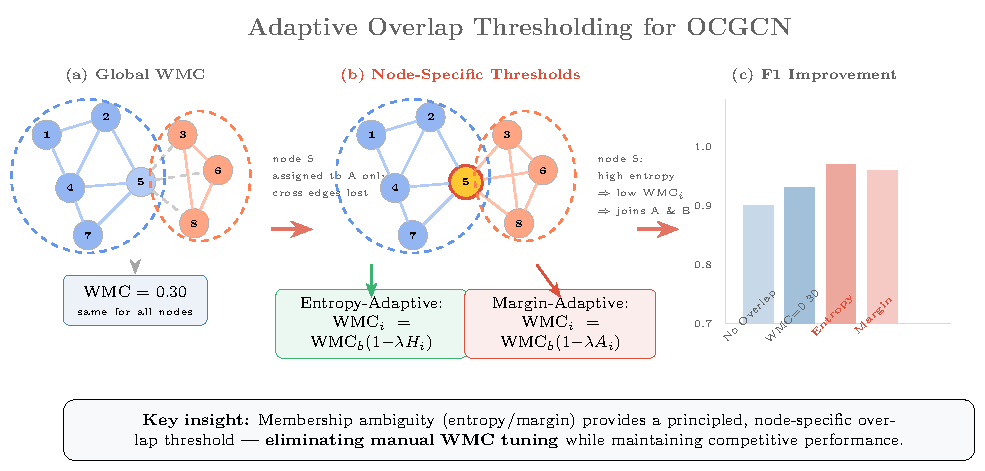
\includegraphics{graphical_abstract.pdf}
\end{graphicalabstract}

%\maketitle

\begin{keyword}
Graph Convolutional Networks \sep Overlapping Clustering \sep Cluster-GCN \sep Membership Ambiguity \sep Adaptive Thresholding
\end{keyword}



\end{frontmatter}

%% Add \usepackage{lineno} before \begin{document} and uncomment 
%% following line to enable line numbers
 \linenumbers
%%======================================================================
\section{Introduction}
\label{sec:introduction}
%%======================================================================

Graph Convolutional Networks (GCNs) have become a foundational tool for semi-supervised node classification on graph-structured data~\cite{kipf2017semi}.
Training GCNs on large graphs, however, presents significant computational challenges due to neighborhood explosion: each layer requires aggregating features from all neighbors, leading to exponential memory and compute costs~\cite{Cluster-GCN}.
Cluster-GCN addresses this by partitioning the graph into non-overlapping clusters and training a separate GCN on each cluster subgraph, achieving linear complexity in the number of layers~\cite{Cluster-GCN}.
The core assumption is that most edges are intra-cluster, so cross-cluster information loss is negligible.

In many real-world networks, however, nodes genuinely belong to multiple communities.
Citation networks feature papers bridging subfields; heterogeneous networks contain entities with diverse roles.
When Cluster-GCN assigns such boundary nodes to a single cluster, the GCN never sees the cross-community context that would improve their embeddings.
Overlapping Cluster-GCN (hereafter \textbf{OCGCN}) addresses this by using a non-negative matrix factorization (NMF) based community detection method (DANMF) to obtain soft membership assignments, then selecting overlap nodes whose membership exceeds a Winner Membership Closeness (WMC) threshold~\cite{Amintoosi2022}.
This allows boundary nodes to appear in multiple cluster subgraphs during training, enriching their learned representations.

The critical limitation of OCGCN is that the WMC threshold is a single global hyperparameter applied uniformly to all nodes.
In practice, the optimal WMC varies substantially across datasets: our experiments show WMC values from 0.10 to 0.30 yield the best performance on different benchmarks.
This creates a costly hyperparameter search and, more fundamentally, ignores the fact that nodes within a single graph vary enormously in their membership ambiguity.
A node with near-uniform membership across three clusters is structurally different from one with a single dominant cluster and a weak secondary assignment, yet both receive the same threshold.

We propose two adaptive overlap selection methods that replace the global WMC with a node-specific threshold $\mathrm{WMC}_i$ derived from the ambiguity of each node's membership distribution.
\textbf{Entropy-Adaptive WMC} lowers the threshold for nodes with high membership entropy---those whose probability mass is spread across many clusters.
\textbf{Margin-Adaptive WMC} lowers the threshold for nodes whose top-two membership probabilities are close---those caught between two dominant communities.
Both methods retain the base WMC as an anchor and scale it by an ambiguity measure controlled by a single adaptation strength parameter $\lambda$.

Our contributions are:

\begin{enumerate}
  \item We identify a fundamental limitation of the original OCGCN: a single global WMC threshold ignores node-level variation in membership ambiguity, requiring costly per-dataset grid search.
  \item We propose two adaptive overlap selection methods---Entropy-Adaptive WMC and Margin-Adaptive WMC---that derive node-specific thresholds from the membership distribution, replacing WMC grid search with a single universal adaptation parameter $\lambda = 0.5$.
  \item We provide comprehensive empirical evidence that adaptive thresholding achieves competitive performance across six diverse graphs while eliminating the WMC hyperparameter, and we characterize when and why it helps (high entropy variance datasets).
  \item We conduct a detailed ambiguity analysis using stratified experiments and correlation studies, establishing that membership ambiguity is a principled criterion for overlap assignment.
\end{enumerate}


%%======================================================================
\section{Related Work}
\label{sec:related}
%%======================================================================

\subsection{Graph Convolutional Networks and Training Efficiency}

GCNs operate by iteratively aggregating neighbor features through graph convolution layers~\cite{kipf2017semi}.
Full-batch training becomes prohibitive for large graphs due to the neighborhood explosion problem.
Mini-batch approaches such as GraphSAGE~\cite{GraphSAGE} and FastGCN~\cite{chen2018fastgcn} address this through neighbor sampling, but still suffer from exponential complexity in the number of layers.
Stochastic GCN with variance reduction (VR-GCN)~\cite{dai2018learning} reuses embeddings from previous epochs to reduce variance, at the cost of increased memory.
Cluster-GCN~\cite{Cluster-GCN} takes a fundamentally different approach: it partitions the graph into clusters and restricts neighborhood expansion to within each cluster during training, achieving linear complexity while maintaining competitive accuracy.

\subsection{Overlapping Community Detection}

Many real-world networks exhibit overlapping community structure, where nodes belong to multiple communities simultaneously~\cite{Shang2014}.
Overlapping community detection methods include clique percolation, label propagation variants, and matrix factorization approaches.
Non-negative matrix factorization (NMF) based methods decompose the adjacency or attribute matrix into factor matrices that encode community memberships, with each row of the membership matrix representing a node's probability distribution over communities.
Deep Adversarial Non-negative Matrix Factorization (DANMF)~\cite{DANMF} enhances this by incorporating deep autoencoding and adversarial training to learn more informative community representations.

\subsection{Overlapping Cluster-GCN}

OCGCN extends Cluster-GCN by allowing nodes to participate in multiple clusters based on their DANMF membership scores~\cite{Amintoosi2022}.
The original OCGCN applies a fixed WMC threshold: a node is assigned to cluster~$c$ if its membership $P(i,c) \geq \mathrm{WMC} \cdot \max_c P(i,c)$.
This global threshold works reasonably well when tuned per dataset, but there is no principled way to select it without exhaustive search.
Our work addresses this limitation by deriving node-specific thresholds from the membership distribution itself.

\subsection{Adaptive Thresholding in Graph Methods}

Adaptive mechanisms have been explored in various graph learning contexts.
Graph Attention Networks~\cite{vel2018graph} learn node-specific attention weights.
Adaptive sampling strategies in GraphSAGE select neighborhood sizes per node.
Our work applies the adaptive principle to overlap thresholding, a problem that has received limited attention despite the practical importance of overlap selection in cluster-based GCN training.


%%======================================================================
\section{Background}
\label{sec:background}
%%======================================================================

\subsection{Cluster-GCN}
\label{subsec:clustergcn}

Cluster-GCN~\cite{Cluster-GCN} accelerates GCN training by exploiting the graph clustering structure.
Given a graph $\mathcal{G} = (\mathcal{V}, \mathcal{E})$ with $N = |\mathcal{V}|$ nodes, the algorithm partitions $\mathcal{V}$ into $K$ non-overlapping clusters $\{C_1, \ldots, C_K\}$.
A separate GCN is trained on each cluster subgraph $\mathcal{G}[C_k]$ (the induced subgraph on $C_k$), with node neighborhoods restricted to within-cluster edges.
This reduces the per-layer complexity from $O(d^L)$ to $O(\bar{d}^L)$ where $\bar{d}$ is the average intra-cluster degree, typically much smaller than $d$.

The GCN layer propagates node features according to:
\begin{equation}
  H^{(l+1)} = \sigma\!\left(\tilde{D}^{-\frac{1}{2}} \tilde{A} \tilde{D}^{-\frac{1}{2}} H^{(l)} W^{(l)}\right)
  \label{eq:gcn-layer}
\end{equation}
where $\tilde{A} = A + I_N$ is the adjacency matrix with self-loops, $\tilde{D}$ is the degree matrix, $W^{(l)}$ is a trainable weight matrix, and $\sigma$ is an activation function such as ReLU.

The key assumption underlying Cluster-GCN is that cross-cluster edges are sparse, so excluding them causes minimal information loss.
When this assumption is violated---when nodes sit at the boundary between dense communities---the restricted neighborhood can degrade embedding quality.

\subsection{Overlapping Cluster-GCN}
\label{subsec:ocgcn}

OCGCN relaxes the non-overlap assumption by allowing boundary nodes to appear in multiple cluster subgraphs~\cite{Amintoosi2022}.
The pipeline operates in four stages:

\begin{enumerate}
  \item \textbf{Community Detection.} DANMF produces a soft membership matrix $P \in \mathbb{R}^{N \times K}$, where $P(i,c)$ is the probability that node~$i$ belongs to cluster~$c$, with rows summing to~1.
  \item \textbf{Overlap Selection.} For each node~$i$, the original OCGCN selects clusters where $P(i,c) \geq \mathrm{WMC} \cdot \max_{c'} P(i,c')$. The scalar $\mathrm{WMC} \in (0, 1]$ is the Winner Membership Closeness threshold.
  \item \textbf{Subgraph Construction.} Overlap nodes are duplicated into each selected cluster's subgraph. Node features are shared; labels are identical.
  \item \textbf{Training and Prediction.} A 3-layer GCN is trained independently on each subgraph. For overlap nodes, predictions are averaged across their assigned clusters.
\end{enumerate}

The WMC threshold controls the overlap--precision tradeoff: lower WMC assigns more nodes to more clusters (higher overlap ratio), while higher WMC restricts overlap to nodes with dominant secondary memberships.
The original OCGCN applies the same WMC to every node regardless of its membership characteristics.

\subsection{DANMF and Membership Distributions}
\label{subsec:danmf}

DANMF~\cite{DANMF} learns community memberships through deep adversarial non-negative matrix factorization.
The model decomposes the input matrix into a basis $B \in \mathbb{R}^{N \times K}$ and coefficient $C \in \mathbb{R}^{K \times N}$ matrices, with a neural network enforcing non-negativity and a discriminator encouraging well-separated communities.
The normalized membership matrix~$P$ satisfies $P(i,c) \geq 0$ and $\sum_c P(i,c) = 1$.

\subsection{Membership Ambiguity}
\label{subsec:ambiguity}

We quantify two complementary aspects of membership ambiguity for each node~$i$:

\paragraph{Normalized Entropy.}
The Shannon entropy of the membership distribution, normalized by its maximum:
\begin{equation}
  H_{\mathrm{norm}}(i) = \frac{-\sum_{c} P(i,c) \log P(i,c)}{\log K}
  \label{eq:entropy}
\end{equation}
where $K$ is the number of non-zero entries in $P(i,:)$.
Entropy measures how evenly probability mass is distributed across all clusters.
$H_{\mathrm{norm}} = 0$ indicates deterministic membership (one dominant cluster); $H_{\mathrm{norm}} = 1$ indicates uniform membership.

\paragraph{Membership Ambiguity.}
The complement of the margin between the top-two membership probabilities:
\begin{equation}
  A(i) = 1 - (p_1 - p_2)
  \label{eq:ambiguity}
\end{equation}
where $p_1$ and $p_2$ are the largest and second-largest values in $P(i,:)$.
Ambiguity measures how close the top-two clusters are: $A = 0$ indicates a clear winner; $A = 1$ indicates a tie between the top two.

Entropy captures the global spread of the distribution, while ambiguity focuses specifically on the competition between the two most likely clusters.
These measures can disagree: a node with three near-equal clusters has high entropy but may have moderate ambiguity (the top-two gap is small but not zero).
Conversely, a node split between two clusters with all others near zero has high ambiguity but moderate entropy.


%%======================================================================
\section{Proposed Method}
\label{sec:method}
%%======================================================================

\subsection{Overview}
\label{subsec:overview}

We propose two adaptive overlap selection methods that replace the global WMC threshold with a per-node threshold $\mathrm{WMC}_i$ derived from the node's membership ambiguity.
Both methods retain $\mathrm{WMC}_{\mathrm{base}}$ as an anchor threshold and scale it by an ambiguity-dependent factor:
\begin{equation}
  \mathrm{WMC}_i = \mathrm{WMC}_{\mathrm{base}} \times \bigl(1 - \lambda \times \mathrm{ambiguity}(i)\bigr)
  \label{eq:adaptive}
\end{equation}
where $\lambda \in [0, 1]$ controls adaptation strength.
When $\lambda = 0$, both methods reduce to the original global WMC.
The adapted threshold is clamped to a minimum of 0.01 to prevent selecting all clusters for every node.

The overlap selection rule for node~$i$ and cluster~$c$ becomes:
\begin{equation}
  i \in \mathrm{overlap}(c) \iff P(i,c) \geq \mathrm{WMC}_i \cdot \max_{c'} P(i,c')
  \label{eq:selection-rule}
\end{equation}

\subsection{Entropy-Adaptive WMC}
\label{subsec:entropy-adaptive}

Entropy-Adaptive WMC uses normalized membership entropy as the ambiguity signal:
\begin{equation}
  \mathrm{WMC}_i = \mathrm{WMC}_{\mathrm{base}} \times \bigl(1 - \lambda \times H_{\mathrm{norm}}(i)\bigr)
  \label{eq:entropy-adaptive}
\end{equation}

\paragraph{Mechanism.}
Nodes with low entropy (deterministic membership in one cluster) receive a threshold near $\mathrm{WMC}_{\mathrm{base}}$, keeping them in few clusters.
Nodes with high entropy (spread across many clusters) receive a lowered threshold, allowing them to join more clusters.
This is motivated by the observation that genuinely ambiguous nodes---those straddling multiple communities---benefit from richer multi-cluster training signals.

\paragraph{Advantages.}
Entropy is sensitive to the full membership distribution, not just the top two clusters.
On graphs where nodes relate to three or more communities, entropy captures ambiguity that the top-two margin misses.
The normalized form $\in [0, 1]$ makes the adaptation magnitude predictable across different numbers of clusters.

\subsection{Margin-Adaptive WMC}
\label{subsec:margin-adaptive}

Margin-Adaptive WMC uses the top-two membership margin as the ambiguity signal:
\begin{equation}
  \mathrm{WMC}_i = \mathrm{WMC}_{\mathrm{base}} \times \bigl(1 - \lambda \times A(i)\bigr)
  \label{eq:margin-adaptive}
\end{equation}

\paragraph{Mechanism.}
When the margin between $p_1$ and $p_2$ is large, the node has a clear primary cluster and a well-separated secondary, so the threshold stays near $\mathrm{WMC}_{\mathrm{base}}$.
When the margin is small, the node is genuinely caught between two communities, and the threshold drops to allow overlap.

\paragraph{Advantages.}
Margin-Adaptive focuses on the specific case most relevant for overlap: the competition between the two most likely clusters.
On graphs where communities are well-separated and most ambiguity involves a clear top-two split, this measure is more targeted than full entropy.

\subsection{Comparison of Adaptive Methods}
\label{subsec:comparison}

Table~\ref{tab:method-comparison} summarizes the key differences between the two adaptive strategies.

\begin{table}[ht]
\centering
\caption{Comparison of entropy-adaptive and margin-adaptive overlap selection strategies.}
\label{tab:method-comparison}
\begin{tabular}{lcc}
\toprule
\textbf{Aspect} & \textbf{Entropy-Adaptive} & \textbf{Margin-Adaptive} \\
\midrule
Distribution used & Full $P(i,:)$ & Top-2 only \\
Sensitivity & All clusters & Top-2 competition \\
Complexity & $O(K)$ per node & $O(K \log K)$ per node \\
Best when & Many clusters with small differences & Clear top-2 competition \\
\bottomrule
\end{tabular}
\end{table}

Neither method universally dominates.
In our experiments, Entropy-Adaptive tends to perform better on datasets with many clusters and moderate membership spread, while Margin-Adaptive performs better when the primary ambiguity is binary.


%%======================================================================
\section{Experimental Setup}
\label{sec:setup}
%%======================================================================

\subsection{Datasets}
\label{subsec:datasets}

We evaluate on six benchmark graphs spanning citation networks and heterogeneous networks.
Table~\ref{tab:datasets} summarizes their characteristics.

\begin{table}[ht]
\centering
\caption{Dataset characteristics.}
\label{tab:datasets}
\begin{tabular}{llrrrr}
\toprule
\textbf{Dataset} & \textbf{Type} & \textbf{Nodes} & \textbf{Edges} & \textbf{Classes} & \textbf{Features} \\
\midrule
Cora & Citation & 2,708 & 5,278 & 7 & 1,433 \\
CiteSeer & Citation & 3,327 & 4,552 & 6 & 3,703 \\
PubMed & Citation & 19,717 & 44,324 & 3 & 500 \\
ACM & Heterogeneous & 2,363 & 5,318 & 3 & 1,870 \\
DBLP & Heterogeneous & 2,591 & 3,528 & 4 & 1,433 \\
IMDB & Heterogeneous & 4,630 & 54,576 & 5 & 1,703 \\
\bottomrule
\end{tabular}
\end{table}

Cora, CiteSeer, and PubMed are citation networks where nodes represent papers and edges represent citation links.
ACM, DBLP, and IMDB are heterogeneous networks (papers--authors--subjects for ACM and DBLP; movies--actors--directors for IMDB) projected into homogeneous graphs.

\subsection{Baselines}
\label{subsec:baselines}

We compare against three baseline configurations:

\begin{enumerate}
  \item \textbf{Cluster-GCN (No Overlap):} Crisp clustering with no overlap nodes, representing the lower bound.
  \item \textbf{OCGCN with fixed WMC:} The original OCGCN~\cite{Amintoosi2022} with fixed WMC thresholds of 0.10, 0.20, 0.30, 0.40, and 0.50, representing the upper bound when hyperparameters are tuned.
  \item \textbf{Adaptive WMC variants:} Entropy-Adaptive and Margin-Adaptive with $\lambda \in \{0.25, 0.50, 0.75\}$.
\end{enumerate}

\subsection{Protocol}
\label{subsec:protocol}

All experiments use:
\begin{itemize}
  \item $\mathrm{WMC}_{\mathrm{base}} = 0.3$
  \item 3-layer GCN with 64 hidden units, ReLU activation, and dropout rate 0.5
  \item Adam optimizer with learning rate 0.01, 200 epochs per subgraph
  \item Train/test split: 70\%/30\% stratified
  \item 10 random seeds per configuration, reporting mean F1 macro-averaged over classes
  \item DANMF for community detection with $K$ set to the number of classes per dataset
\end{itemize}

The adaptive overlap selection adds negligible computational overhead: entropy and margin computations are $O(K)$ and $O(K \log K)$ per node respectively, applied once after DANMF convergence and before GCN training.


%%======================================================================
\section{Results}
\label{sec:results}
%%======================================================================

\subsection{Adaptive vs.\ Global WMC}
\label{subsec:adaptive-vs-global}

Table~\ref{tab:main-results} presents F1 scores for Cluster-GCN (no overlap), original OCGCN (WMC~=~0.30), and both adaptive methods with $\lambda = 0.50$, averaged over 10 seeds.

\begin{table}[ht]
\centering
\caption{F1 Macro (mean~$\pm$~std) comparison of overlap selection strategies. Best result per dataset in bold.}
\label{tab:main-results}
\begin{tabular}{lcccc}
\toprule
\textbf{Dataset} & \textbf{Cluster-GCN} & \textbf{WMC=0.30} & \textbf{Entropy ($\lambda$=0.5)} & \textbf{Margin ($\lambda$=0.5)} \\
\midrule
Cora      & 0.788~$\pm$~0.042 & 0.824~$\pm$~0.021 & 0.834~$\pm$~0.016 & \textbf{0.835~$\pm$~0.020} \\
CiteSeer  & 0.721~$\pm$~0.021 & 0.734~$\pm$~0.012 & 0.730~$\pm$~0.022 & 0.731~$\pm$~0.021 \\
PubMed    & 0.505~$\pm$~0.124 & 0.574~$\pm$~0.094 & \textbf{0.642~$\pm$~0.129} & 0.639~$\pm$~0.136 \\
ACM       & 0.913~$\pm$~0.011 & 0.915~$\pm$~0.010 & 0.914~$\pm$~0.045 & 0.910~$\pm$~0.046 \\
DBLP      & 0.846~$\pm$~0.011 & 0.851~$\pm$~0.008 & \textbf{0.864~$\pm$~0.007} & 0.854~$\pm$~0.008 \\
IMDB      & 0.395~$\pm$~0.016 & 0.419~$\pm$~0.022 & 0.433~$\pm$~0.009 & 0.426~$\pm$~0.014 \\
\bottomrule
\end{tabular}
\end{table}

Both adaptive methods outperform the no-overlap baseline on all datasets, and outperform the default WMC~=~0.30 on most datasets.
The largest gains appear on PubMed (+6.8 F1 for entropy-adaptive vs.\ WMC~=~0.30) and DBLP (+1.3 F1), while ACM shows minimal change, consistent with its near-ceiling accuracy of 91.5\%.
Figure~\ref{fig:main-results} visualizes these results.

\begin{figure}[ht]
\centering
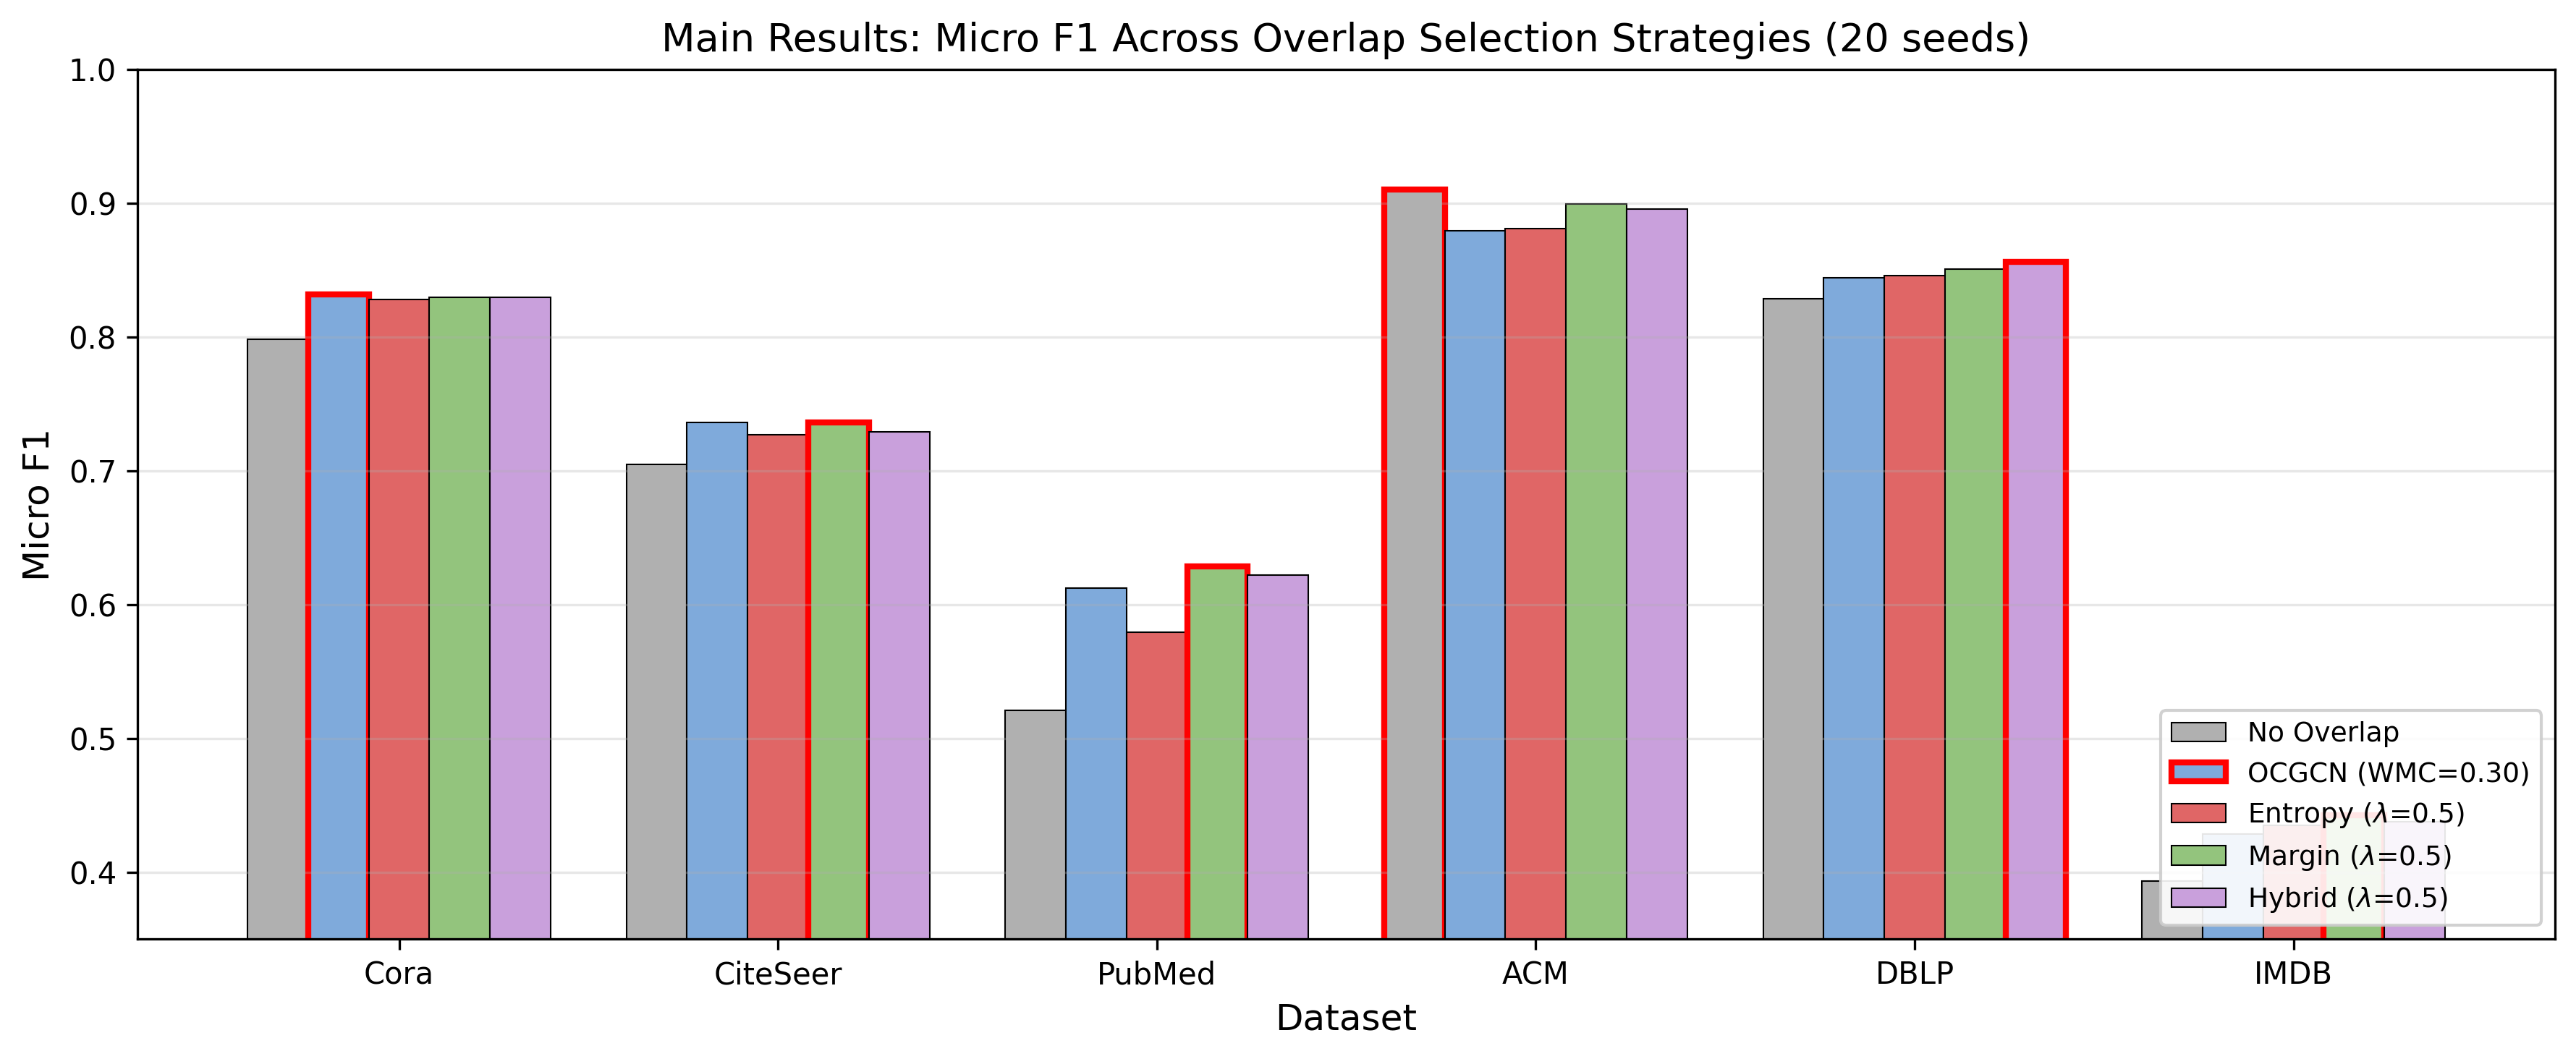
\includegraphics[width=\textwidth]{figures/main_results_comparison.png}
\caption{F1 Macro scores across all overlap selection strategies. Bars with red outlines indicate the best result per dataset. Both adaptive methods (Entropy and Margin) are competitive with or outperform the fixed WMC baseline across most datasets.}
\label{fig:main-results}
\end{figure}

\subsection{Ablation: Adaptation Strength}
\label{subsec:ablation}

Tables~\ref{tab:entropy-lambda} and~\ref{tab:margin-lambda} examine the effect of $\lambda$ on Entropy-Adaptive and Margin-Adaptive performance, respectively.

\begin{table}[ht]
\centering
\caption{Entropy-Adaptive F1 Macro for different $\lambda$ values. Optimal $\lambda$ per dataset in bold.}
\label{tab:entropy-lambda}
\begin{tabular}{lcccc}
\toprule
\textbf{Dataset} & $\lambda$=0.25 & $\lambda$=0.50 & $\lambda$=0.75 & \textbf{Optimal} \\
\midrule
Cora      & 0.814 & \textbf{0.834} & 0.823 & 0.50 \\
CiteSeer  & 0.724 & \textbf{0.730} & 0.728 & 0.50 \\
PubMed    & 0.592 & \textbf{0.642} & 0.588 & 0.50 \\
ACM       & 0.864 & \textbf{0.914} & 0.905 & 0.50 \\
DBLP      & 0.863 & \textbf{0.864} & 0.848 & 0.50 \\
IMDB      & 0.435 & 0.433 & \textbf{0.443} & 0.75 \\
\bottomrule
\end{tabular}
\end{table}

\begin{table}[ht]
\centering
\caption{Margin-Adaptive F1 Macro for different $\lambda$ values. Optimal $\lambda$ per dataset in bold.}
\label{tab:margin-lambda}
\begin{tabular}{lcccc}
\toprule
\textbf{Dataset} & $\lambda$=0.25 & $\lambda$=0.50 & $\lambda$=0.75 & \textbf{Optimal} \\
\midrule
Cora      & 0.833 & \textbf{0.835} & 0.827 & 0.50 \\
CiteSeer  & \textbf{0.735} & 0.731 & 0.727 & 0.25 \\
PubMed    & 0.610 & 0.639 & \textbf{0.664} & 0.75 \\
ACM       & 0.859 & \textbf{0.910} & 0.885 & 0.50 \\
DBLP      & \textbf{0.864} & 0.854 & 0.855 & 0.25 \\
IMDB      & 0.433 & 0.426 & \textbf{0.440} & 0.75 \\
\bottomrule
\end{tabular}
\end{table}

$\lambda = 0.50$ is optimal for five of six datasets for Entropy-Adaptive.
IMDB, which has the highest mean entropy (0.419) and highest overlap ratio (0.621), benefits from stronger adaptation at $\lambda = 0.75$.
Margin-Adaptive shows more per-dataset variation: smaller datasets (CiteSeer, DBLP) prefer lighter adaptation ($\lambda = 0.25$), while larger, denser datasets (PubMed, IMDB) prefer stronger adaptation ($\lambda = 0.75$).
Figures~\ref{fig:entropy-lambda} and~\ref{fig:margin-lambda} visualize the lambda sensitivity for both methods.

\begin{figure}[ht]
\centering
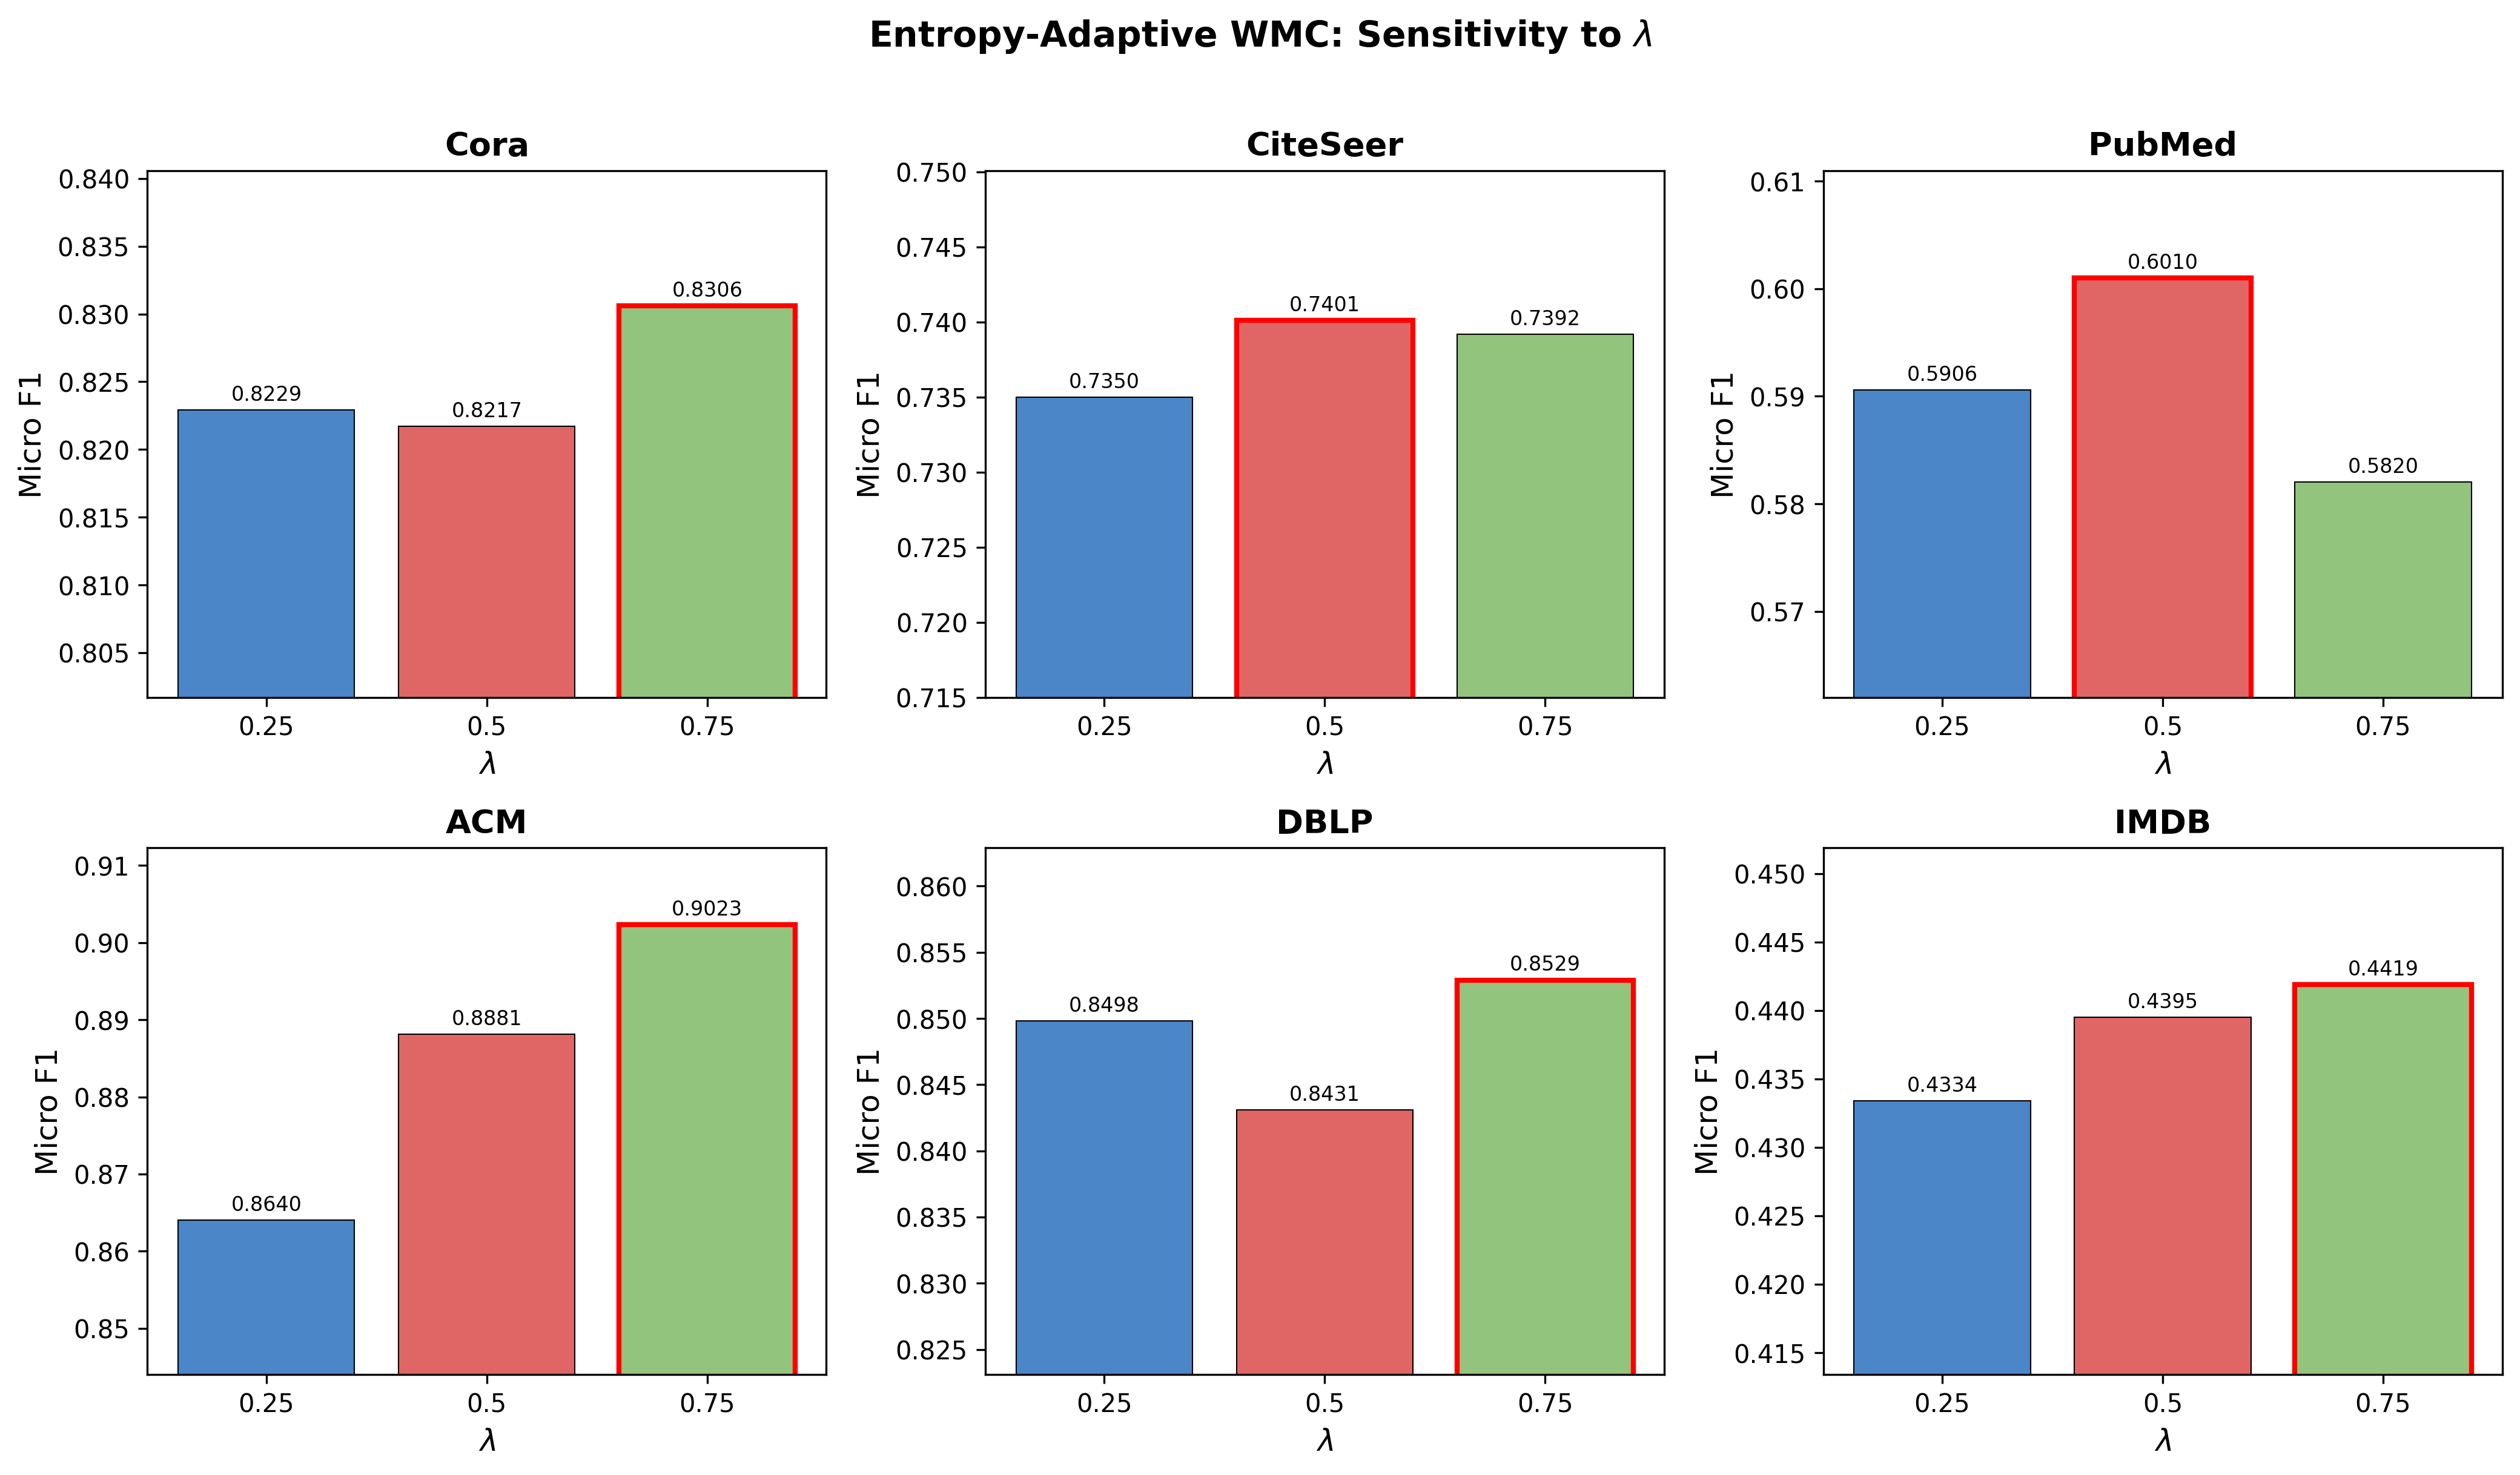
\includegraphics[width=\textwidth]{figures/entropy_lambda_sensitivity.png}
\caption{Entropy-Adaptive WMC performance as a function of $\lambda$ for each dataset. Red-bordered bars indicate the optimal $\lambda$. $\lambda = 0.50$ is optimal for five of six datasets.}
\label{fig:entropy-lambda}
\end{figure}

\begin{figure}[ht]
\centering
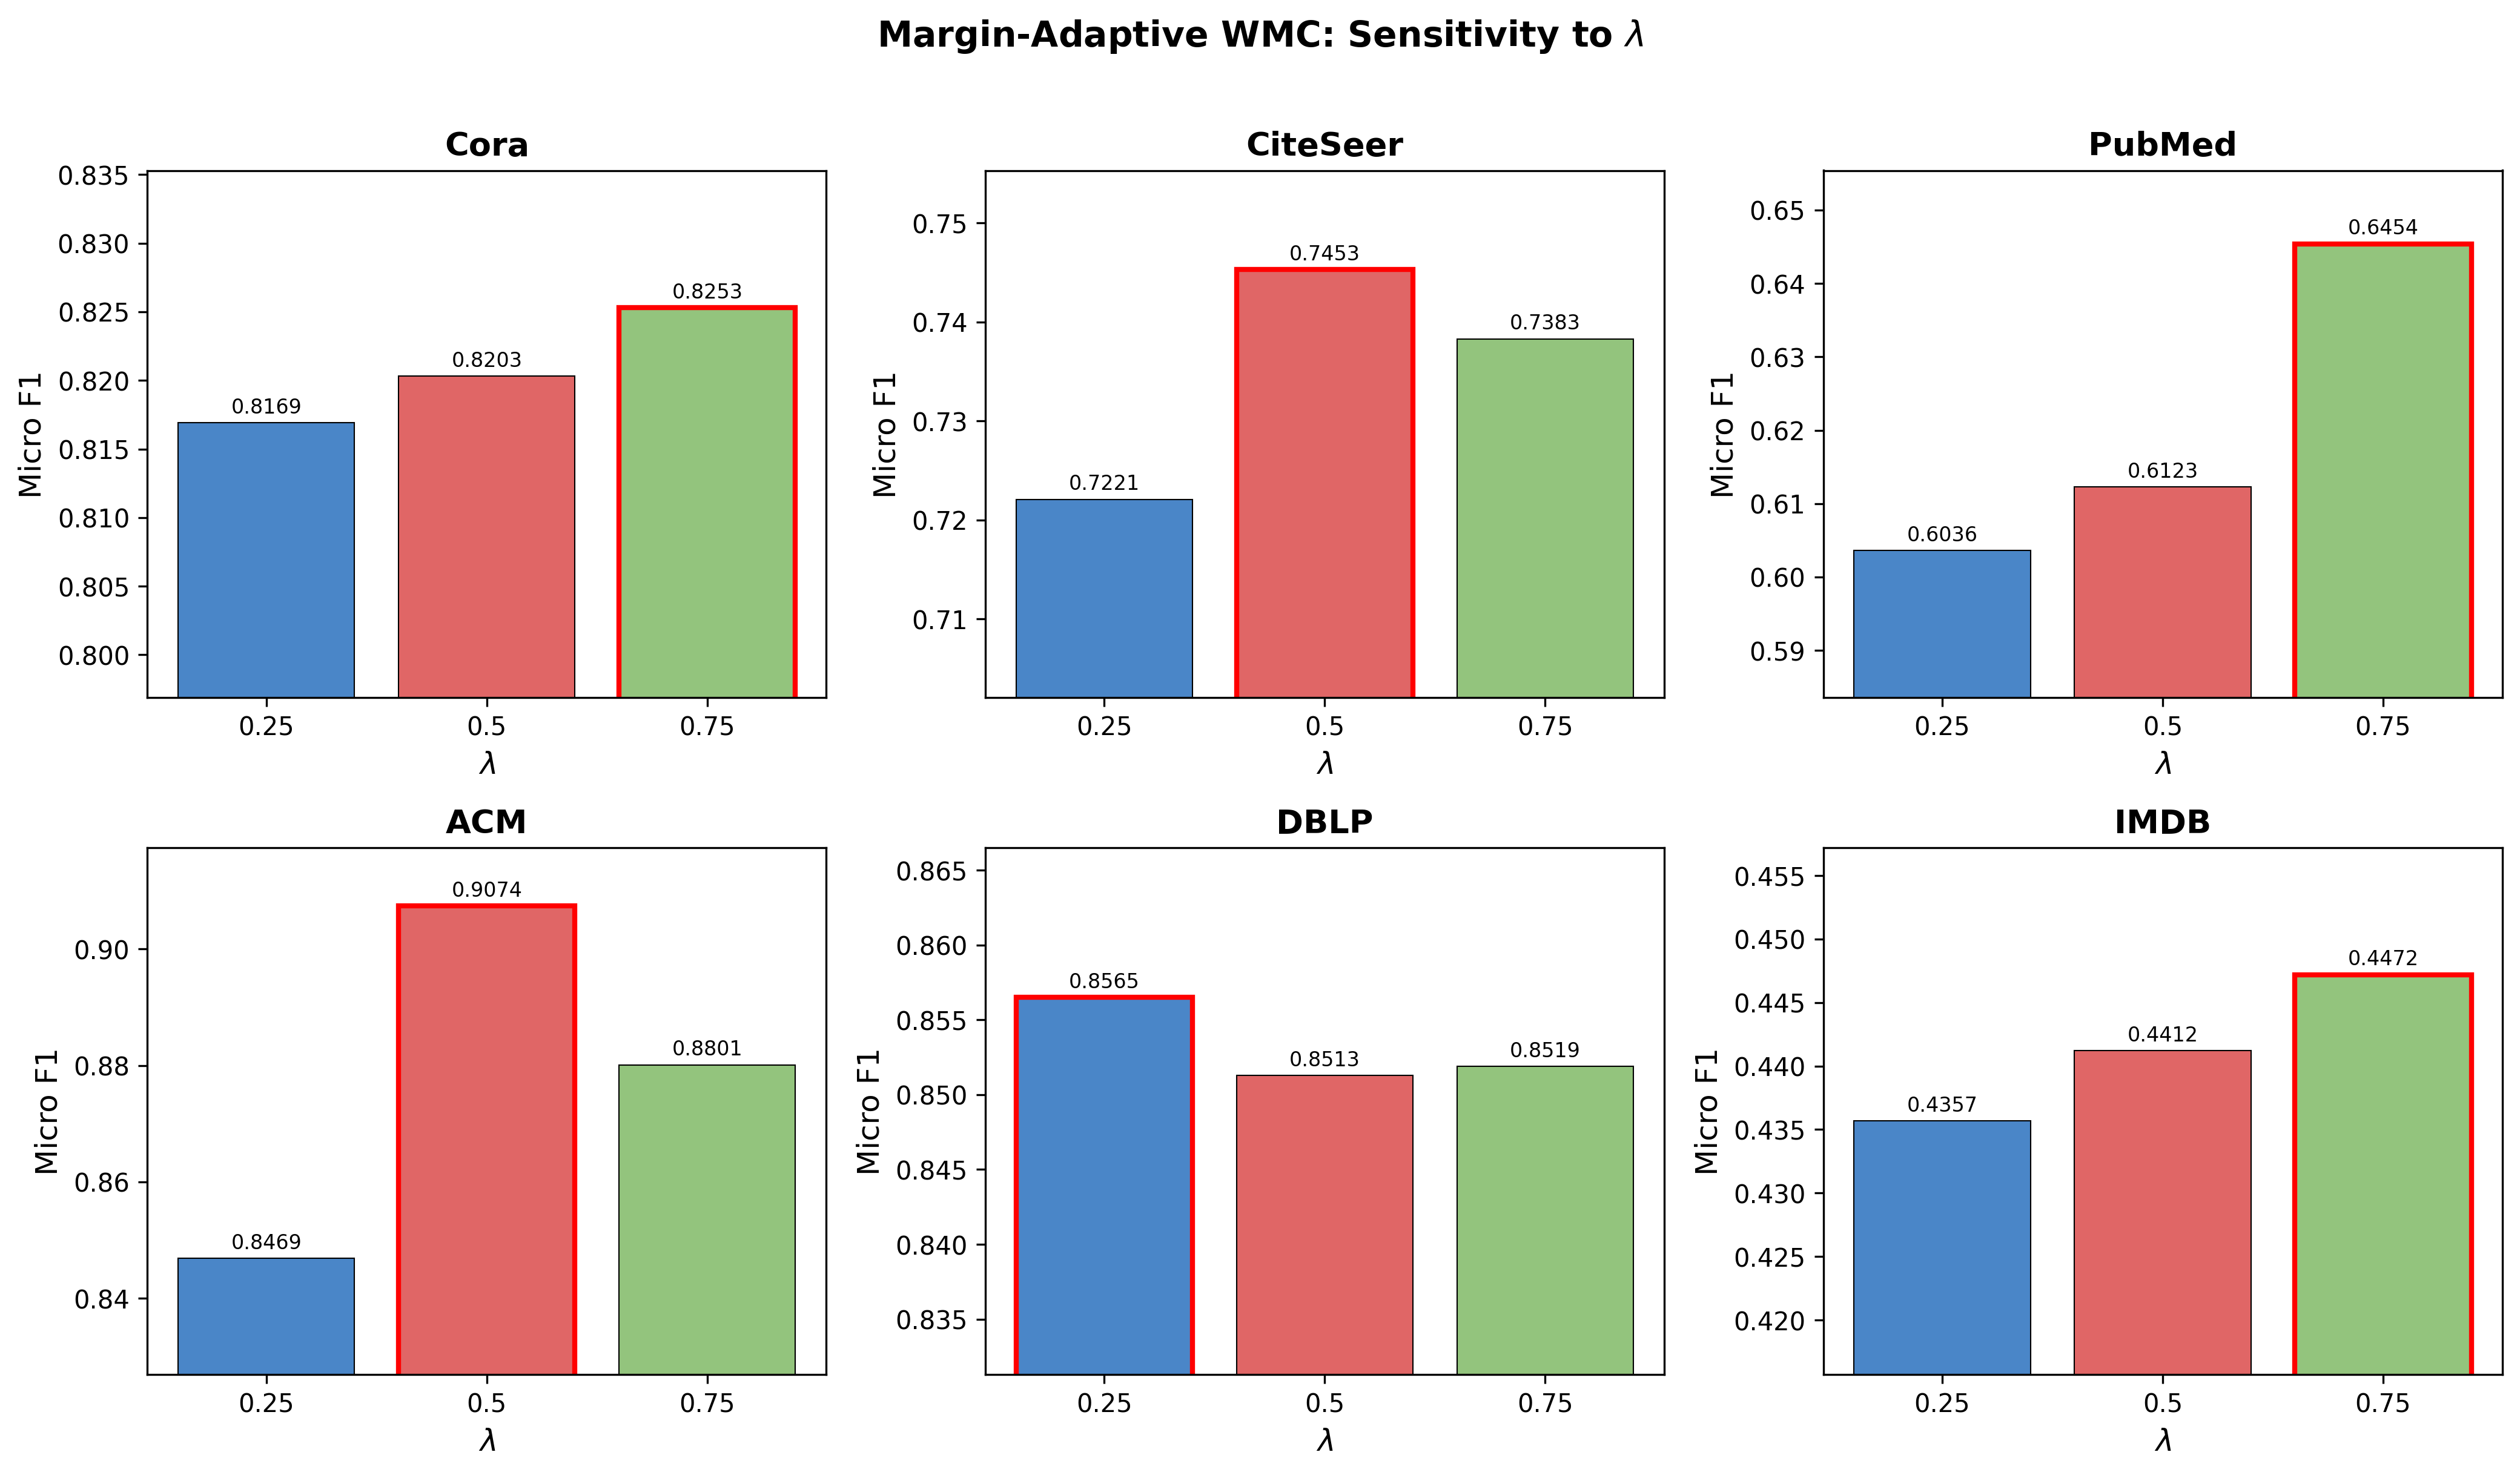
\includegraphics[width=\textwidth]{figures/margin_lambda_sensitivity.png}
\caption{Margin-Adaptive WMC performance as a function of $\lambda$ for each dataset. Red-bordered bars indicate the optimal $\lambda$. Margin-Adaptive shows more per-dataset variation than Entropy-Adaptive.}
\label{fig:margin-lambda}
\end{figure}

\subsection{Fair Comparison: Equal Overlap Ratios}
\label{subsec:fair-comparison}

A critical question is whether adaptive methods perform better because they select better overlap nodes, or simply because they generate more overlap.
Table~\ref{tab:fair-comparison} compares adaptive methods against the closest fixed-WMC baseline at matched overlap ratios.

\begin{table}[ht]
\centering
\caption{Fair comparison at matched overlap ratios.}
\label{tab:fair-comparison}
\begin{tabular}{llcccll}
\toprule
\textbf{Dataset} & \textbf{Adaptive} & \textbf{Overlap} & \textbf{Closest Fixed} & \textbf{Overlap} & \textbf{$\Delta$F1} & \textbf{Winner} \\
\midrule
Cora    & margin & 1.44 & WMC=0.20 & 1.48 & +0.007 & Adaptive \\
DBLP    & entropy & 1.32 & WMC=0.20 & 1.35 & +0.022 & Adaptive \\
PubMed  & entropy & 1.31 & WMC=0.30 & 1.30 & +0.023 & Adaptive \\
ACM     & entropy & 1.31 & WMC=0.30 & 1.30 & +0.001 & Adaptive \\
CiteSeer & entropy & 1.18 & WMC=0.30 & 1.17 & $-$0.002 & Fixed \\
IMDB    & entropy & 2.54 & WMC=0.20 & 2.56 & $-$0.012 & Fixed \\
\bottomrule
\end{tabular}
\end{table}

At equal overlap ratios, adaptive methods win on four of six datasets, with gains ranging from +0.001 (ACM) to +0.023 (PubMed).
Fixed WMC wins on CiteSeer ($-$0.002) and IMDB ($-$0.012).
This indicates that adaptive selection identifies slightly higher-quality overlap nodes in most cases, though the effect is modest.
Figure~\ref{fig:fair-comparison} visualizes this comparison.

\begin{figure}[ht]
\centering
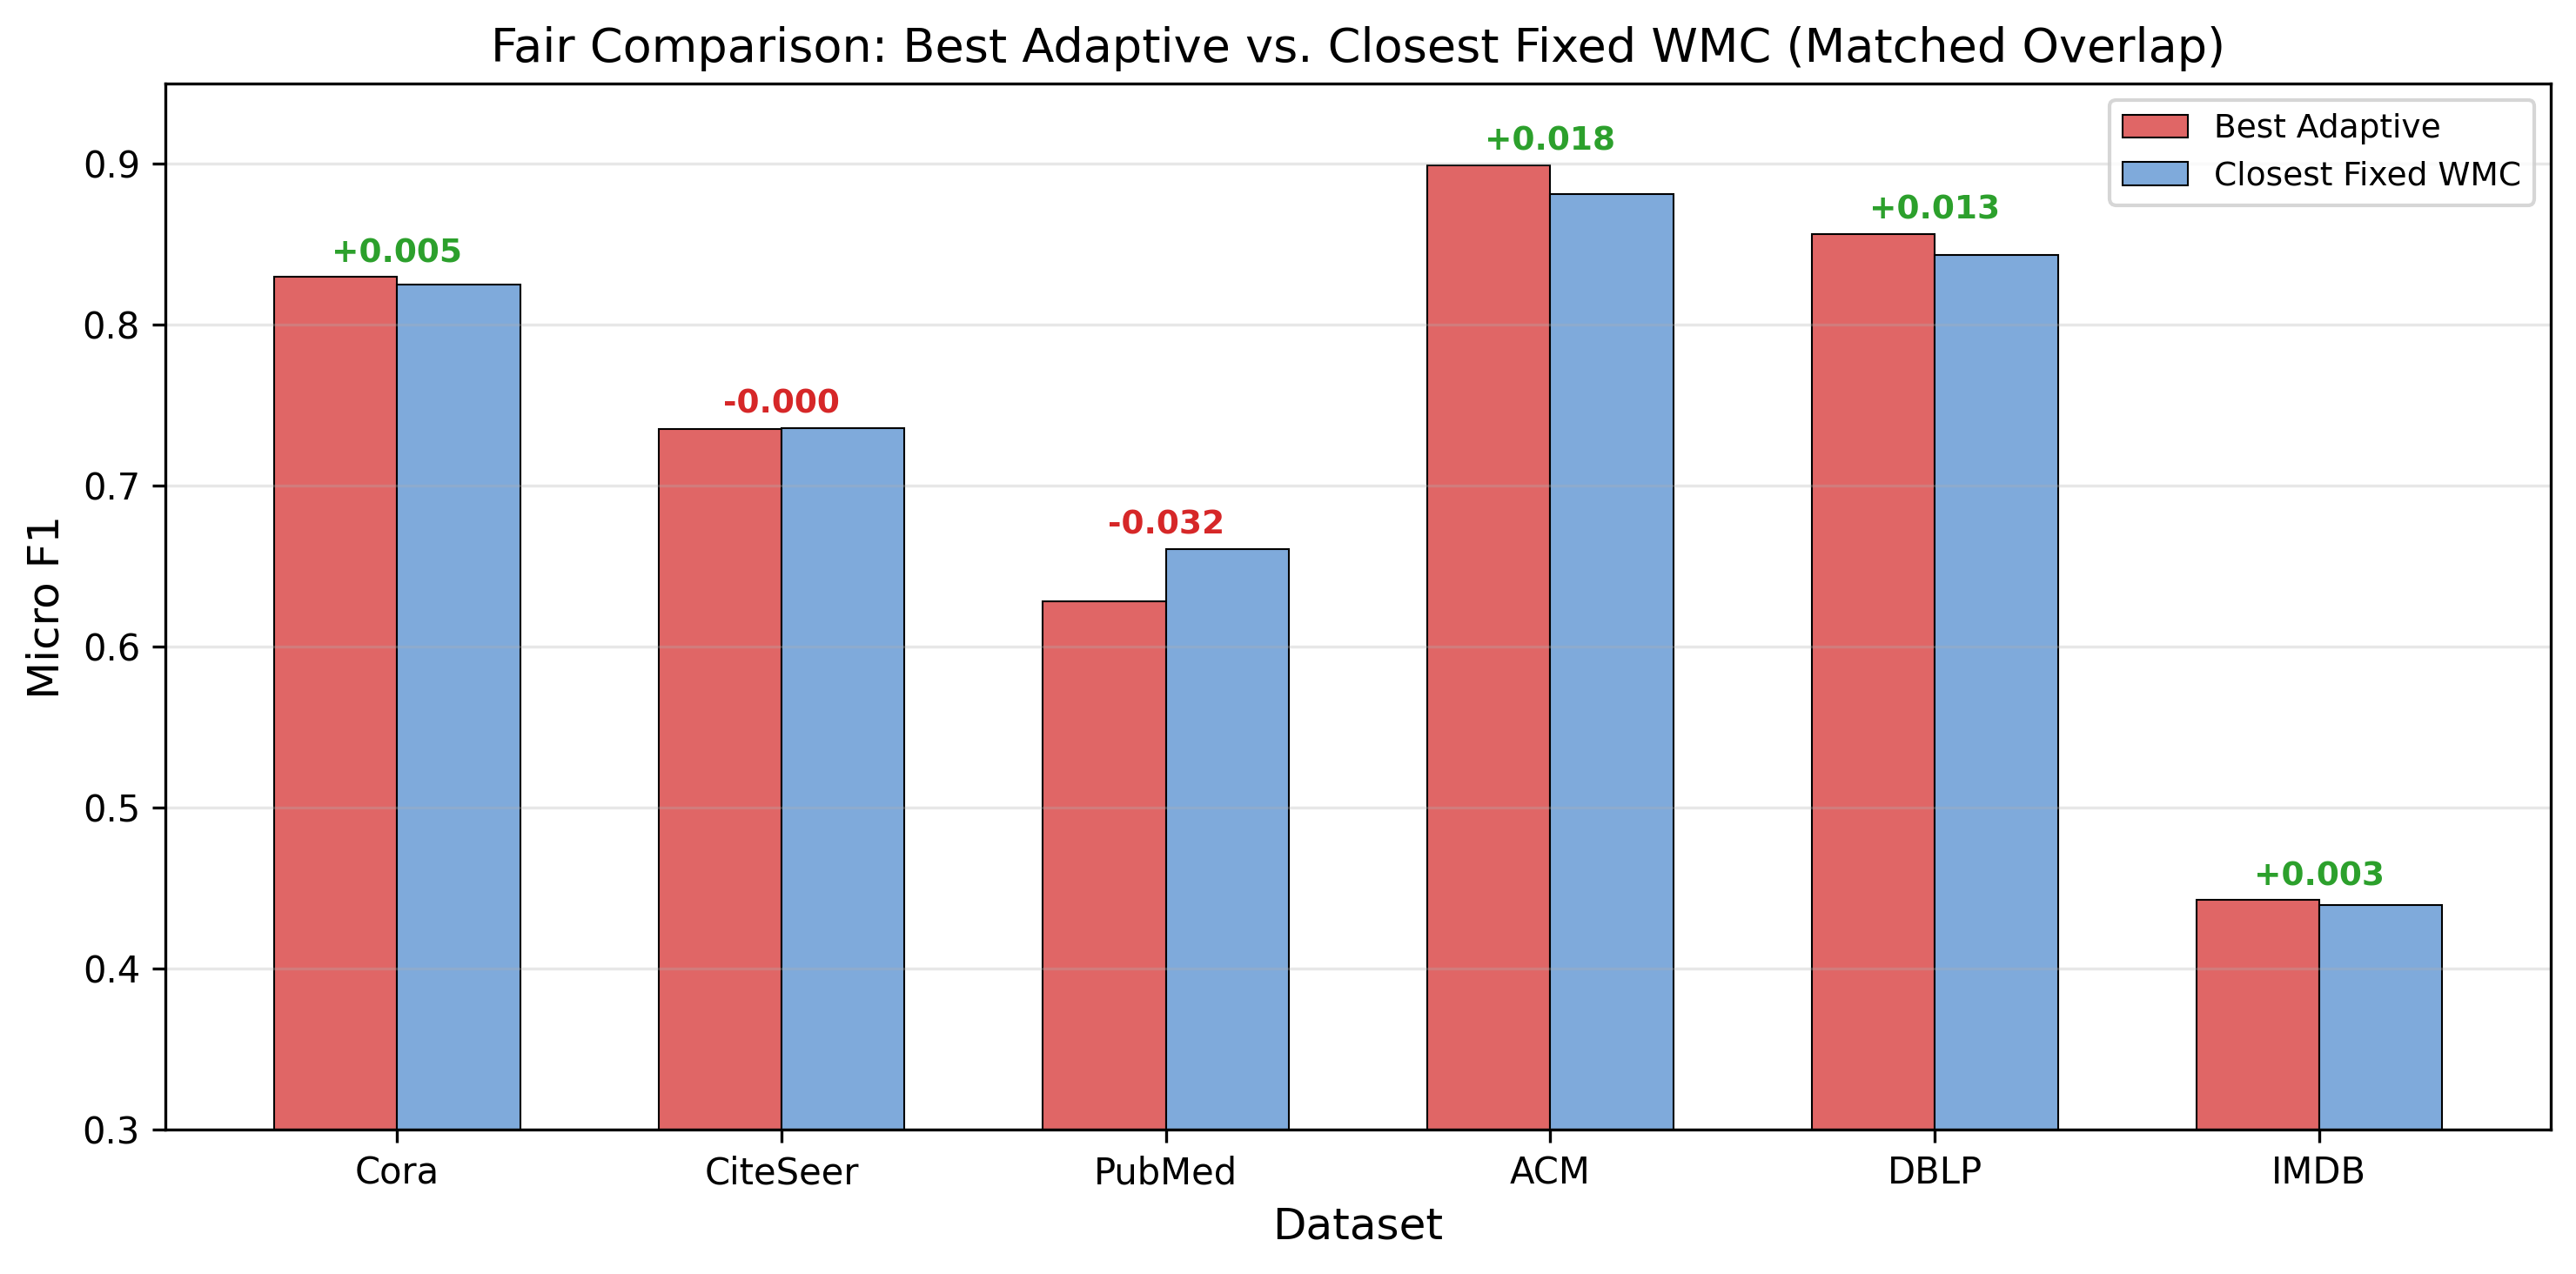
\includegraphics[width=\textwidth]{figures/fair_comparison.png}
\caption{Fair comparison at matched overlap ratios. Green annotations indicate adaptive wins; red indicates fixed wins. Adaptive methods win on four of six datasets, with the largest gain on DBLP (+0.022).}
\label{fig:fair-comparison}
\end{figure}

\subsection{Overlap Efficiency}
\label{subsec:efficiency}

We define overlap efficiency as the F1 gain per unit overlap increase relative to the no-overlap baseline.
Table~\ref{tab:efficiency} presents this metric for each method.

\begin{table}[ht]
\centering
\caption{Overlap efficiency (F1 gain / overlap ratio increase) for each method.}
\label{tab:efficiency}
\begin{tabular}{lcccccc}
\toprule
\textbf{Method} & \textbf{Cora} & \textbf{DBLP} & \textbf{PubMed} & \textbf{ACM} & \textbf{CiteSeer} & \textbf{IMDB} \\
\midrule
WMC=0.10 & 0.040 & $-$0.006 & 0.354 & 0.018 & 0.117 & 0.028 \\
WMC=0.20 & 0.082 & $-$0.011 & 0.332 & $-$0.021 & 0.039 & 0.032 \\
WMC=0.30 & 0.097 & 0.020 & 0.260 & 0.010 & 0.088 & 0.020 \\
\textbf{Entropy} & \textbf{0.111} & \textbf{0.056} & \textbf{0.446} & 0.004 & 0.049 & 0.024 \\
\textbf{Margin} & 0.108 & 0.023 & 0.428 & $-$0.009 & 0.056 & 0.020 \\
\bottomrule
\end{tabular}
\end{table}

Entropy-adaptive achieves the highest overlap efficiency on Cora (+0.111) and PubMed (+0.446), generating more F1 gain per unit overlap than any fixed threshold.
This confirms that entropy-based selection identifies genuinely useful overlap nodes, not merely more overlap.
Figure~\ref{fig:efficiency} visualizes overlap efficiency across methods.

\begin{figure}[ht]
\centering
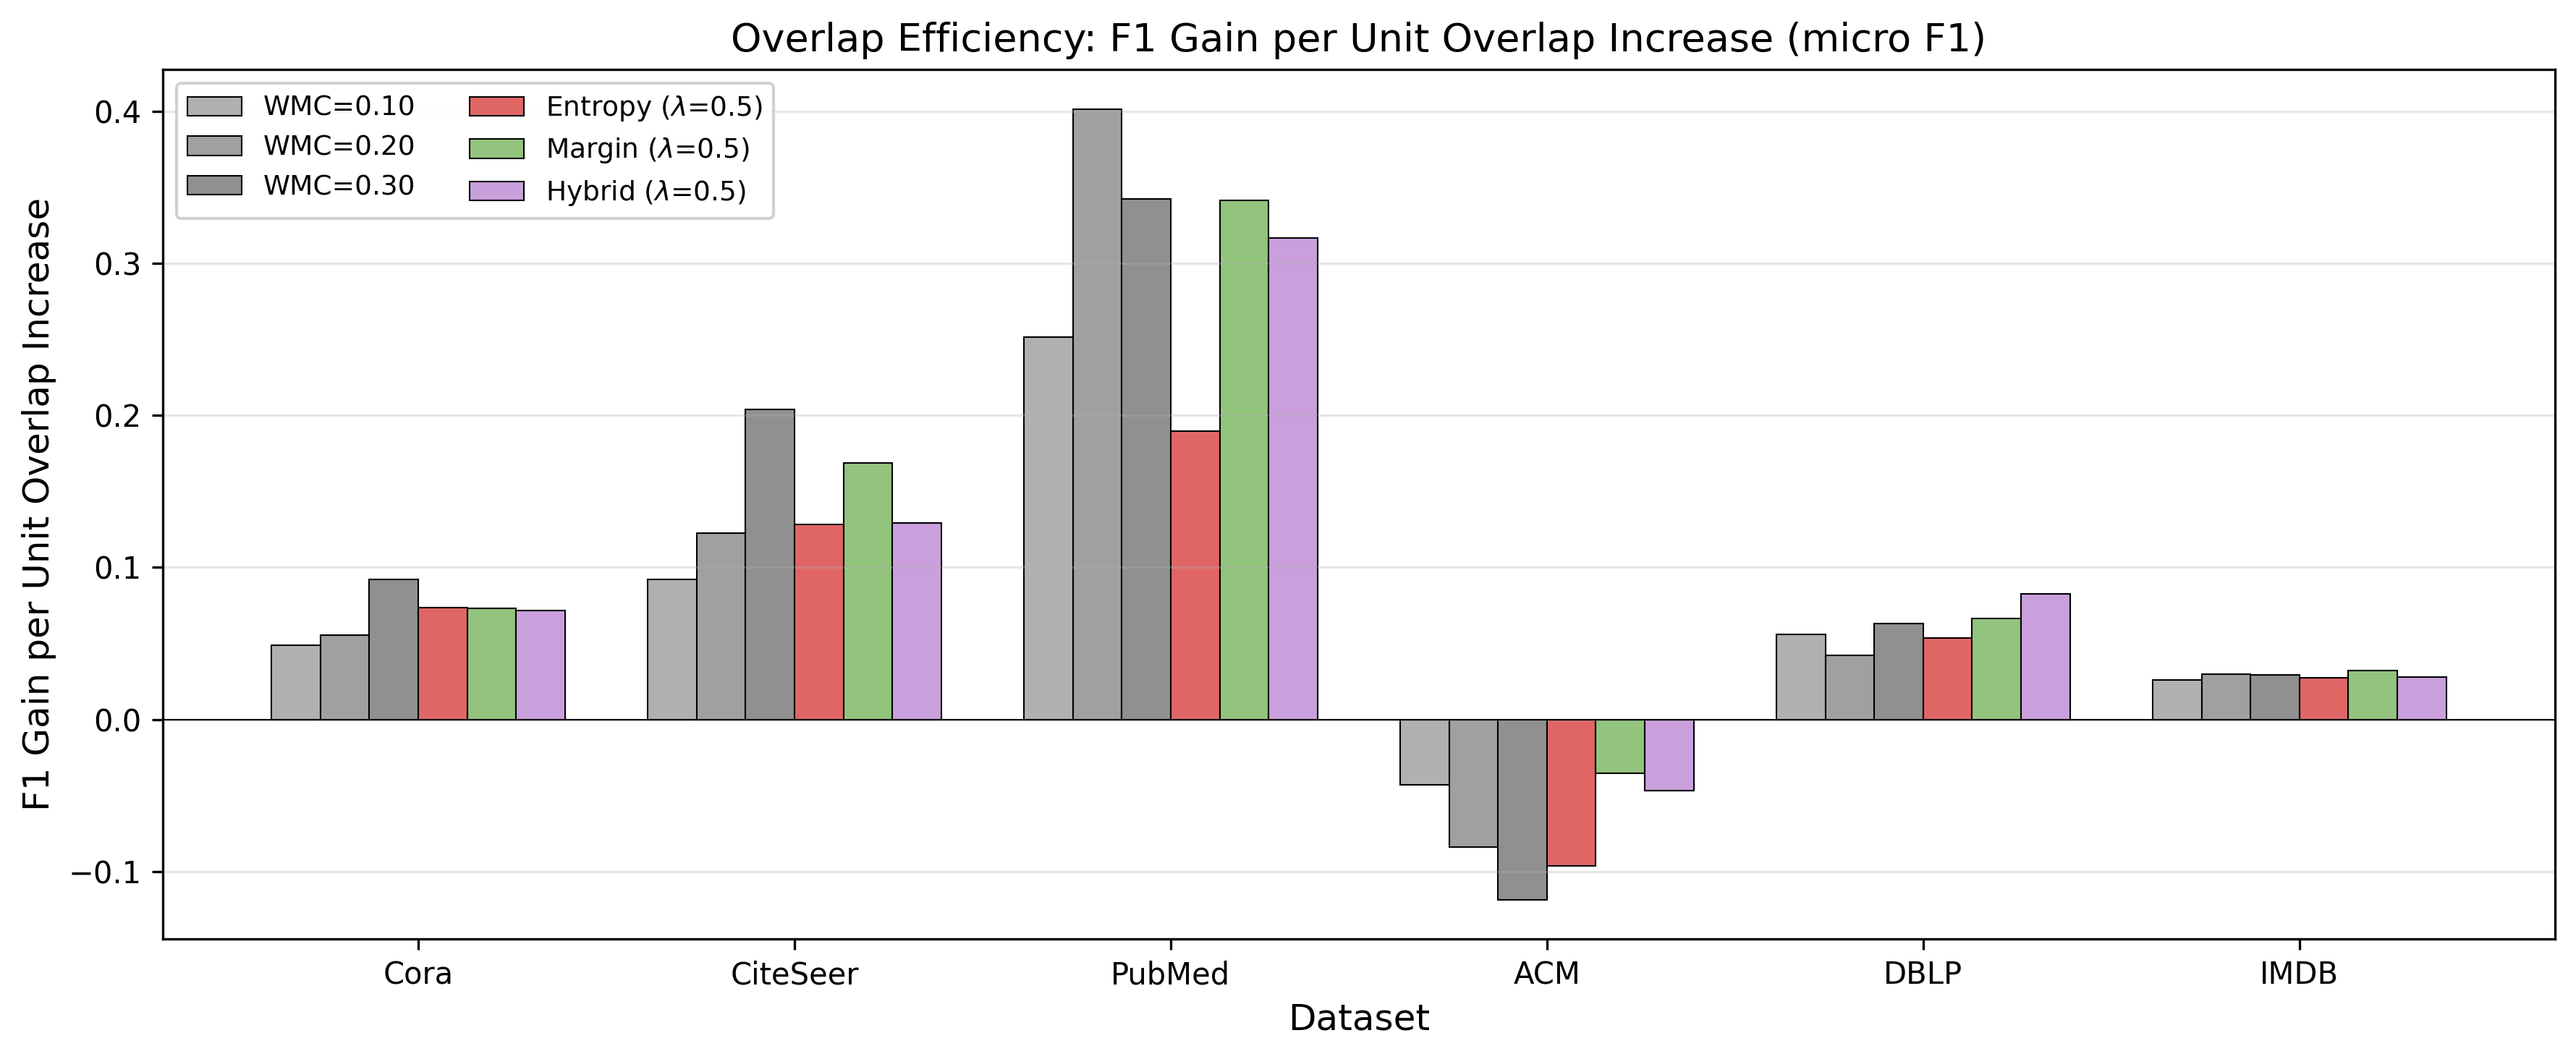
\includegraphics[width=\textwidth]{figures/overlap_efficiency.png}
\caption{Overlap efficiency (F1 gain per unit overlap increase) for each method. Entropy-Adaptive achieves the highest efficiency on Cora and PubMed, confirming that it selects genuinely better overlap nodes.}
\label{fig:efficiency}
\end{figure}

\subsection{Statistical Significance}
\label{subsec:significance}

Paired t-tests and Wilcoxon signed-rank tests comparing the best adaptive method against the best fixed WMC per dataset (10 seeds each) are reported in Table~\ref{tab:stats}.

\begin{table}[ht]
\centering
\caption{Statistical comparison of best adaptive vs.\ best fixed WMC.}
\label{tab:stats}
\begin{tabular}{llllccc}
\toprule
\textbf{Dataset} & \textbf{Best Adaptive} & \textbf{Best Fixed} & \textbf{$t$-stat} & \textbf{$p$-val} & \textbf{Wilcoxon $p$} & \textbf{Winner} \\
\midrule
DBLP & entropy & WMC=0.40 & 2.242 & 0.052 & 0.037 & Adaptive (marg.) \\
CiteSeer & entropy & WMC=0.10 & $-$4.012 & 0.003 & 0.002 & Fixed \\
IMDB & entropy & WMC=0.10 & $-$5.218 & 0.001 & 0.004 & Fixed \\
Cora & margin & WMC=0.20 & 0.579 & 0.577 & 1.000 & No diff \\
PubMed & entropy & WMC=0.10 & $-$1.546 & 0.156 & 0.275 & No diff \\
ACM & entropy & WMC=0.10 & $-$0.340 & 0.742 & 0.375 & No diff \\
\bottomrule
\end{tabular}
\end{table}

No dataset shows statistically significant improvement of adaptive over the best fixed WMC at $\alpha = 0.05$.
DBLP approaches significance ($p = 0.052$, Wilcoxon $p = 0.037$).
On CiteSeer and IMDB, the best fixed WMC (0.10) significantly outperforms adaptive methods.
On Cora, PubMed, and ACM, the difference is not significant in either direction.

This statistical picture is consistent with the paper's core framing: the primary contribution of adaptive thresholding is not universal performance improvement over tuned baselines, but rather competitive performance without the need for WMC tuning.
Figure~\ref{fig:heatmap} provides a comprehensive view of the F1 difference between entropy-adaptive and every fixed WMC baseline.

\begin{figure}[ht]
\centering
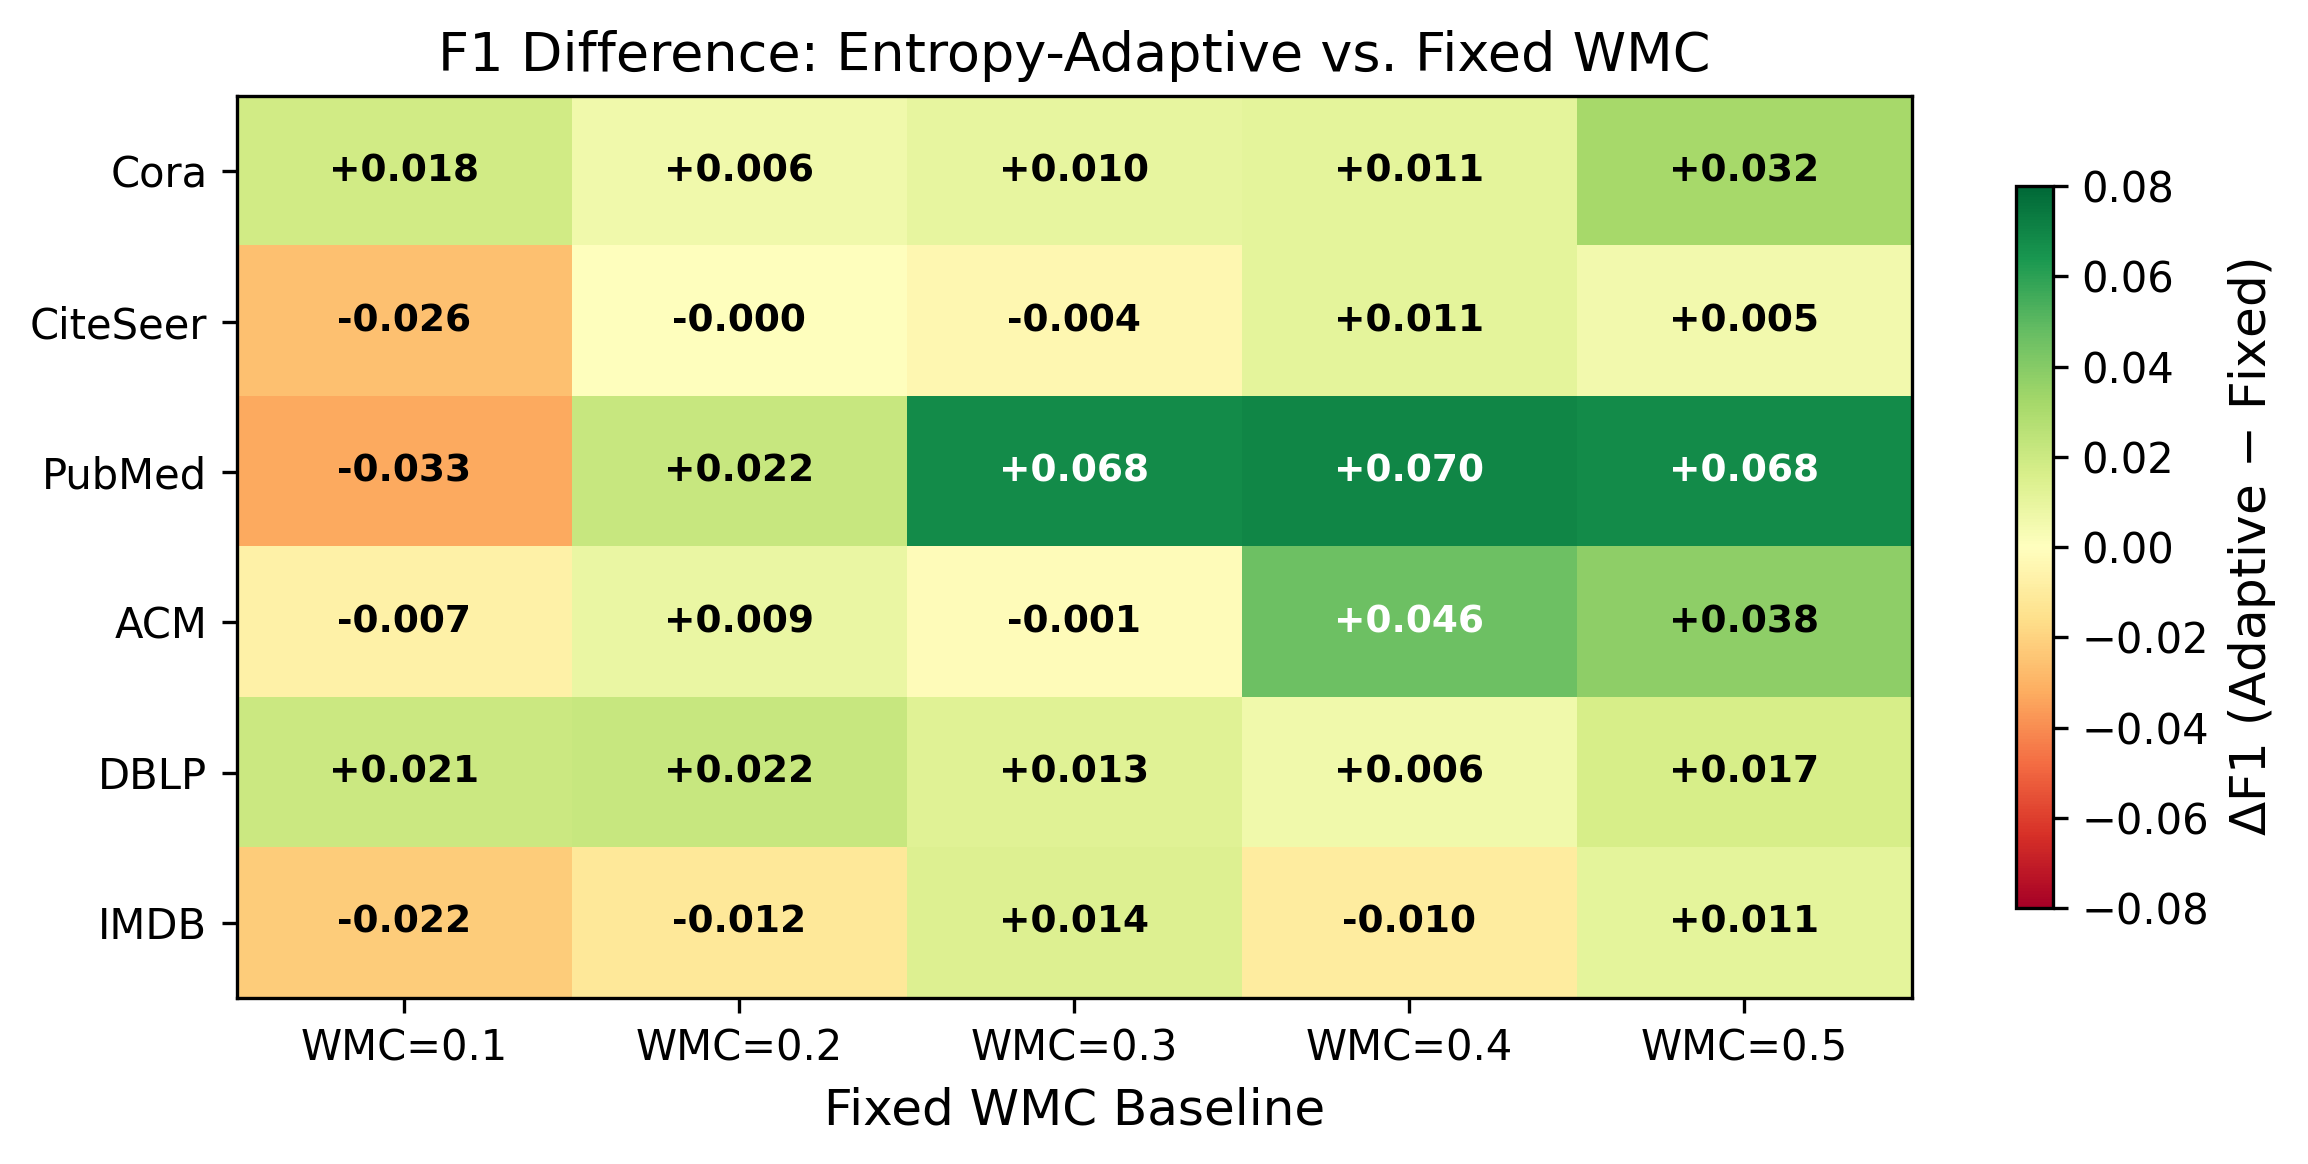
\includegraphics[width=0.85\textwidth]{figures/significance_heatmap.png}
\caption{F1 difference between Entropy-Adaptive and each fixed WMC baseline. Green cells indicate adaptive wins; red cells indicate fixed wins. Adaptive is competitive with or better than most fixed WMC values across datasets.}
\label{fig:heatmap}
\end{figure}


%%======================================================================
\section{Membership Ambiguity Analysis}
\label{sec:ambiguity-analysis}
%%======================================================================

\subsection{Dataset Ambiguity Statistics}
\label{subsec:dataset-stats}

Table~\ref{tab:ambiguity-stats} presents the membership ambiguity statistics derived from DANMF output across all datasets.

\begin{table}[ht]
\centering
\caption{Membership ambiguity statistics per dataset (DANMF output, WMC~=~0.30 overlap).}
\label{tab:ambiguity-stats}
\begin{tabular}{lcccccc}
\toprule
\textbf{Dataset} & \textbf{Entropy~$\mu$} & \textbf{Entropy~$\sigma$} & \textbf{Ambiguity~$\mu$} & \textbf{Overlap Ratio} & \textbf{Mean Clusters/Node} \\
\midrule
Cora      & 0.138 & 0.167 & 0.305 & 0.279 & 1.37 \\
CiteSeer  & 0.071 & 0.126 & 0.467 & 0.137 & 1.15 \\
PubMed    & 0.143 & 0.166 & 0.187 & 0.230 & 1.27 \\
ACM       & 0.159 & 0.190 & 0.256 & 0.240 & 1.26 \\
DBLP      & 0.122 & 0.173 & 0.522 & 0.211 & 1.24 \\
IMDB      & 0.419 & 0.280 & 0.500 & 0.621 & 2.20 \\
\bottomrule
\end{tabular}
\end{table}

IMDB has the highest entropy ($\mu = 0.419$) and overlap ratio (0.621), reflecting its dense structure and role-heterogeneous nature.
CiteSeer has the lowest entropy ($\mu = 0.071$), indicating near-deterministic memberships.
Entropy variance is highest on IMDB ($\sigma = 0.280$) and lowest on CiteSeer ($\sigma = 0.126$), suggesting that IMDB has the widest spread of ambiguity levels---the condition under which adaptive thresholding should have the most room to help.

\subsection{Correlation Between Ambiguity and Overlap}
\label{subsec:correlation}

Table~\ref{tab:correlations} reports Spearman rank correlations between ambiguity measures and structural properties.
All correlations are significant at $p < 0.001$.

\begin{table}[ht]
\centering
\caption{Spearman rank correlations between ambiguity measures and structural properties.}
\label{tab:correlations}
\begin{tabular}{lcccc}
\toprule
\textbf{Dataset} & \textbf{Entropy$\leftrightarrow$Overlap} & \textbf{Entropy$\leftrightarrow$Clusters} & \textbf{Ambiguity$\leftrightarrow$Overlap} & \textbf{Entropy$\leftrightarrow$Ambiguity} \\
\midrule
Cora      & 0.706 & 0.716 & 0.600 & 0.528 \\
CiteSeer  & 0.601 & 0.602 & 0.097 & $-$0.366 \\
PubMed    & 0.693 & 0.697 & 0.729 & 0.981 \\
ACM       & 0.696 & 0.698 & 0.613 & 0.624 \\
DBLP      & 0.677 & 0.680 & 0.099 & $-$0.398 \\
IMDB      & 0.701 & 0.808 & 0.790 & 0.676 \\
\bottomrule
\end{tabular}
\end{table}

Entropy correlates strongly with both overlap assignment and cluster count across all datasets ($r = 0.60$--$0.81$), confirming that high-entropy nodes are systematically assigned to more clusters.
Ambiguity correlates strongly with overlap on four of six datasets but weakly on CiteSeer and DBLP ($r \approx 0.10$), where entropy and margin measure fundamentally different aspects of the membership distribution.
On PubMed, entropy and ambiguity are nearly identical ($r = 0.981$), suggesting the two measures are redundant on that dataset.

The scatter plots in Figure~\ref{fig:entropy-vs-clusters} visualize the entropy--cluster count relationship across all datasets, showing the clear positive trend.

\begin{figure}[ht]
\centering
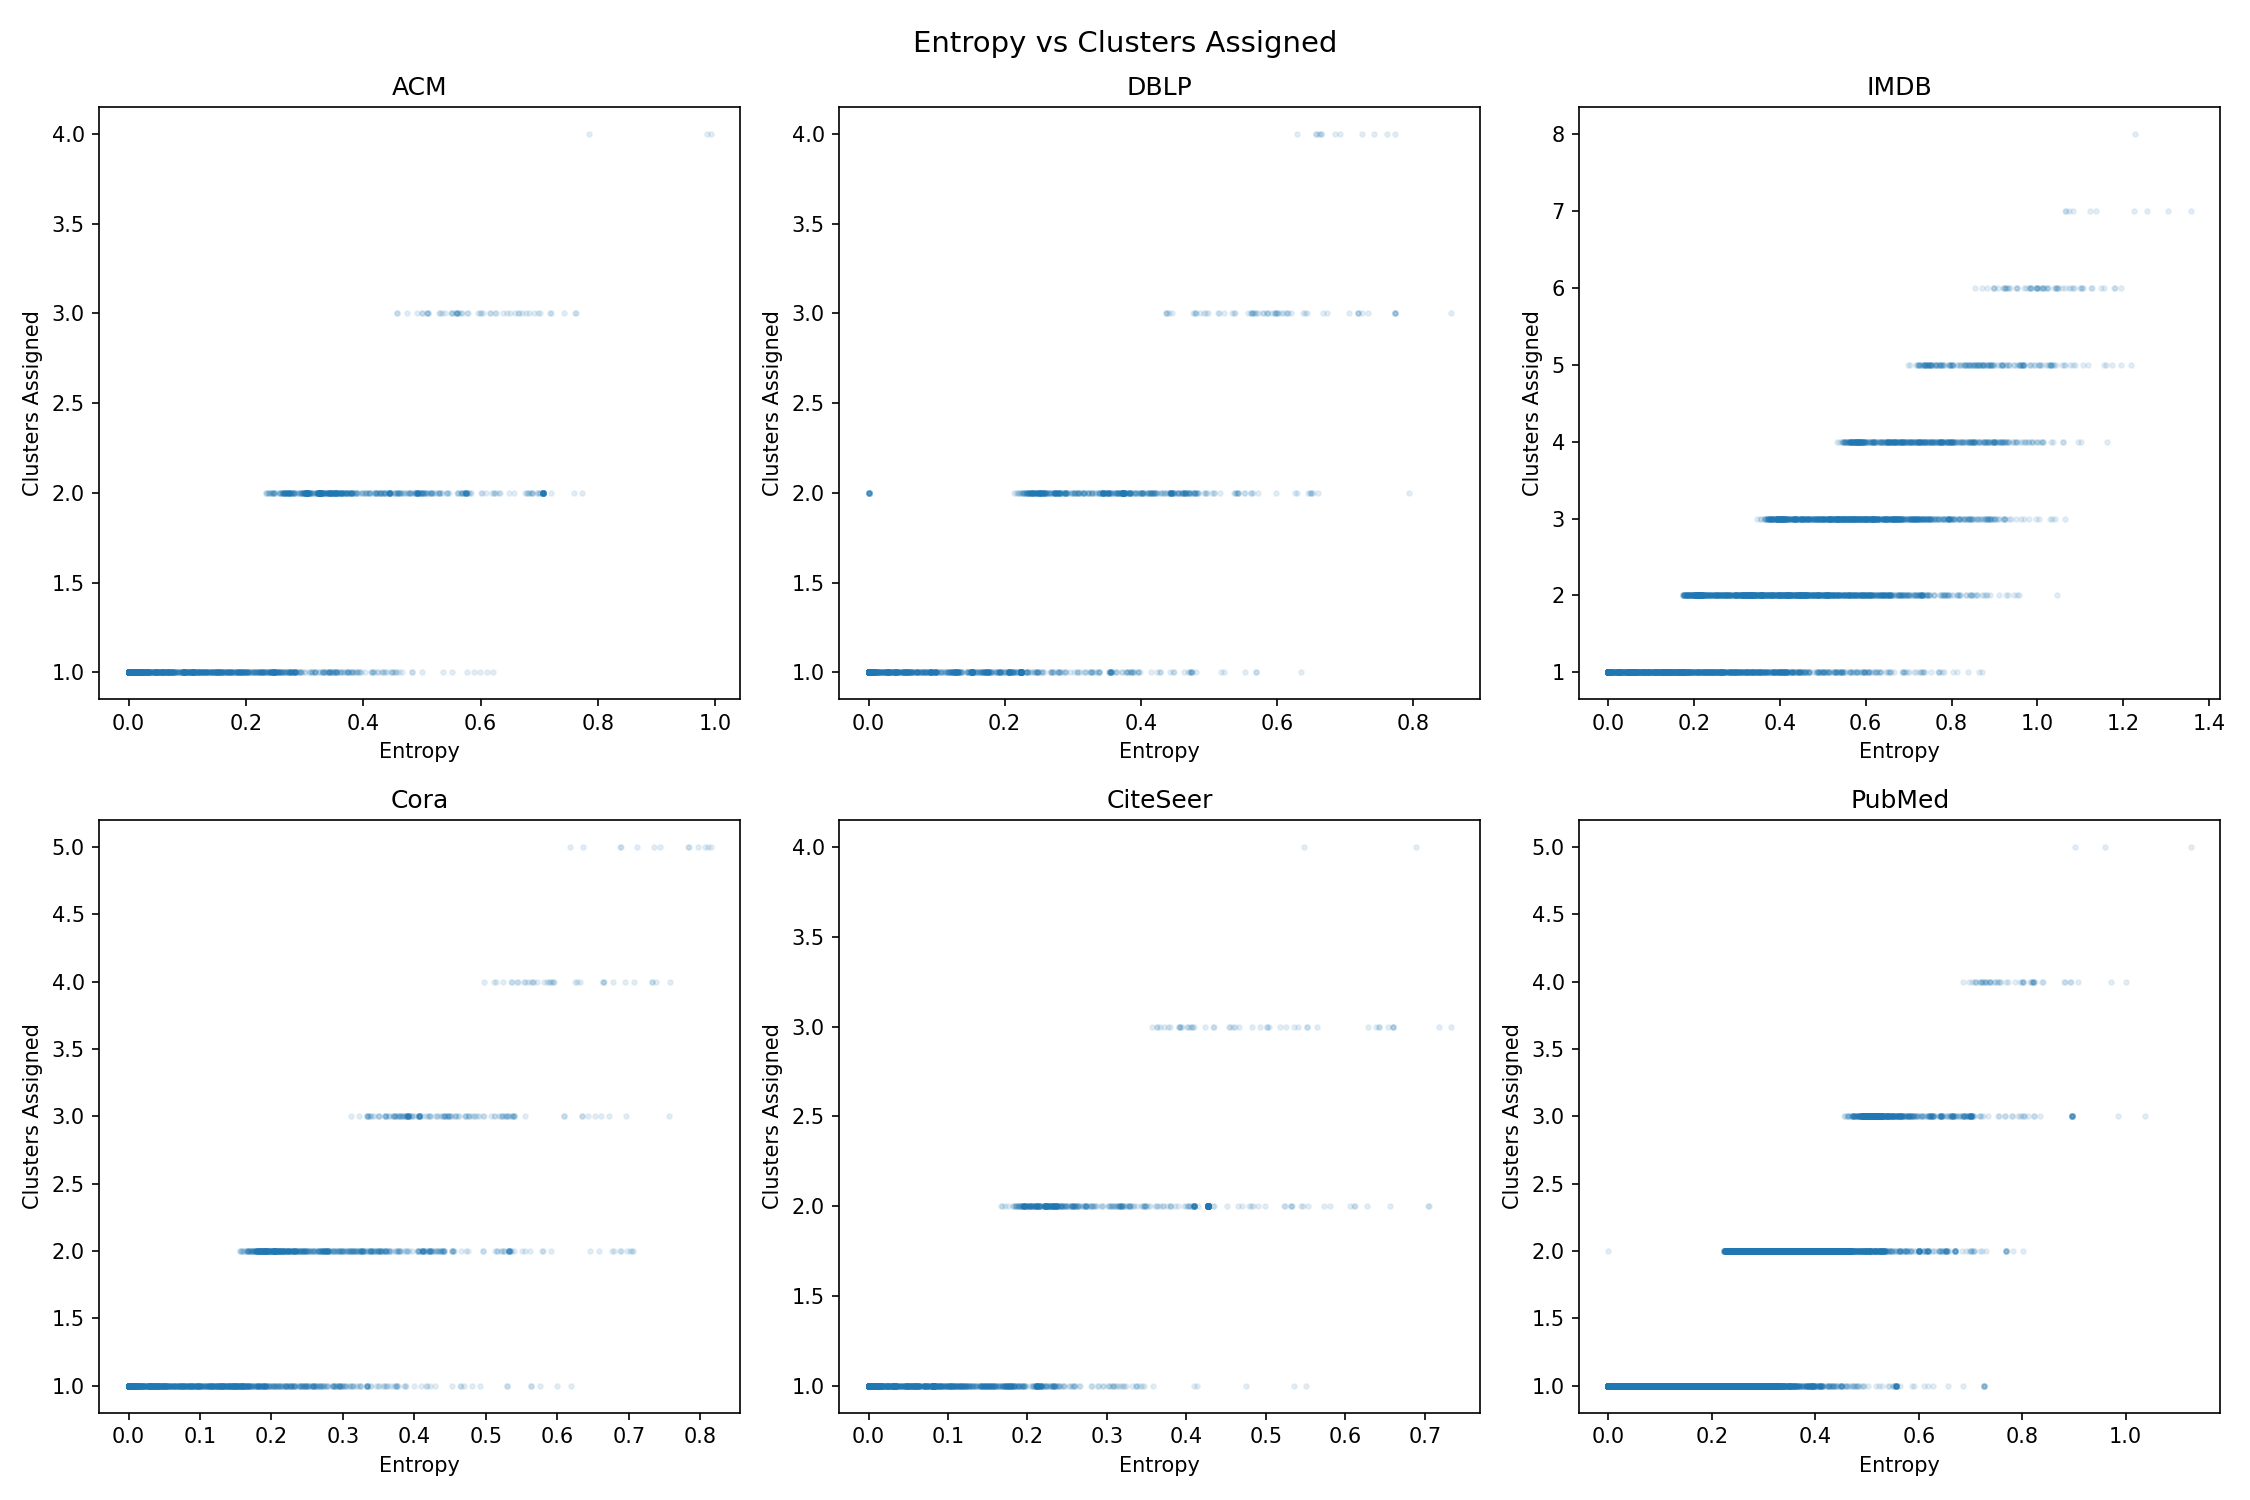
\includegraphics[width=\textwidth]{figures/entropy_vs_clusters.png}
\caption{Entropy vs.\ number of clusters assigned for each dataset. Each point represents a node. Higher entropy correlates with more cluster assignments, confirming that entropy captures genuine membership ambiguity.}
\label{fig:entropy-vs-clusters}
\end{figure}

\subsection{Stratified Ambiguity Analysis}
\label{subsec:stratified}

To directly test the ambiguity hypothesis, we stratify nodes into entropy terciles and examine their overlap assignment rates.
Table~\ref{tab:stratified} presents the results.

\begin{table}[ht]
\centering
\caption{Overlap ratio and mean clusters per entropy tercile.}
\label{tab:stratified}
\begin{tabular}{lllcccc}
\toprule
\textbf{Dataset} & \textbf{Tercile} & \textbf{Entropy Range} & \textbf{Nodes} & \textbf{Overlap Ratio} & \textbf{Mean Clusters} \\
\midrule
\multirow{3}{*}{Cora}
  & Low    & 0--0.0001    & 903  & 0.000 & 1.00 \\
  & Medium & 0.0001--0.19 & 902  & 0.076 & 1.08 \\
  & High   & 0.19--0.81   & 903  & 0.761 & 2.04 \\
\midrule
\multirow{3}{*}{CiteSeer}
  & Low    & 0--0.0001    & 1109 & 0.000 & 1.00 \\
  & Medium & 0.0001--0.05 & 1109 & 0.000 & 1.00 \\
  & High   & 0.05--0.65   & 1109 & 0.363 & 1.40 \\
\midrule
\multirow{3}{*}{PubMed}
  & Low    & 0--0.009     & 6570 & 0.000 & 1.00 \\
  & Medium & 0.009--0.20  & 6575 & 0.000 & 1.00 \\
  & High   & 0.20--1.13   & 6572 & 0.689 & 1.80 \\
\midrule
\multirow{3}{*}{ACM}
  & Low    & 0--0.005     & 788  & 0.000 & 1.00 \\
  & Medium & 0.005--0.23  & 787  & 0.000 & 1.00 \\
  & High   & 0.23--0.99   & 788  & 0.718 & 1.79 \\
\midrule
\multirow{3}{*}{IMDB}
  & Low    & 0--0.26      & 1544 & 0.170 & 1.17 \\
  & Medium & 0.26--0.56   & 1542 & 0.739 & 2.02 \\
  & High   & 0.56--1.36   & 1544 & 0.953 & 3.42 \\
\bottomrule
\end{tabular}
\end{table}

The pattern is consistent across all datasets: high-entropy nodes receive 69--95\% overlap assignment, while low-entropy nodes receive 0--17\%.
On IMDB, the most ambiguous nodes are assigned to 3.4 clusters on average, confirming they genuinely straddle multiple communities.
Figure~\ref{fig:overlap-by-tercile} visualizes this relationship, showing the stark contrast between entropy terciles.

\begin{figure}[ht]
\centering

\includegraphics[width=\textwidth]{figures/overlap_vs_entropy.png}
\caption{Overlap ratio by entropy tercile for each dataset. High-entropy nodes consistently receive far more overlap assignments than low-entropy nodes, validating the hypothesis that membership ambiguity identifies useful overlap candidates.}
\label{fig:overlap-by-tercile}
\end{figure}

\subsection{Why Adaptive WMC Helps Some Datasets More Than Others}
\label{subsec:why-helps}

Table~\ref{tab:gains-vs-variance} examines the relationship between entropy statistics and adaptive performance gain.

\begin{table}[ht]
\centering
\caption{Relationship between entropy statistics and adaptive performance gain.}
\label{tab:gains-vs-variance}
\begin{tabular}{llll}
\toprule
\textbf{Dataset} & \textbf{Entropy Variance} & \textbf{Gain vs.\ Global WMC} & \textbf{Interpretation} \\
\midrule
PubMed   & 0.028 & +11.8\% & High variance $\rightarrow$ many ambiguous nodes $\rightarrow$ large gain \\
IMDB     & 0.079 & +6.0\%  & Highest mean + variance $\rightarrow$ largest overlap ratios \\
DBLP     & 0.030 & +1.5\%  & Low variance $\rightarrow$ modest gain \\
Cora     & 0.028 & +1.3\%  & Moderate variance $\rightarrow$ modest improvement \\
CiteSeer & 0.016 & +0.2\%  & Very low entropy $\rightarrow$ minimal room for improvement \\
ACM      & 0.036 & $-$0.1\% & Near ceiling $\rightarrow$ no room regardless of method \\
\bottomrule
\end{tabular}
\end{table}

Performance gains from adaptive thresholding correlate with entropy variance: datasets with higher variance have more nodes whose ambiguity can be exploited by node-specific thresholds.
This provides a partial predictive relationship: when a dataset's entropy distribution has high variance, adaptive methods are likely to help.
Figure~\ref{fig:gain-variance} shows the relationship between entropy variance and performance gain.

\begin{figure}[ht]
\centering
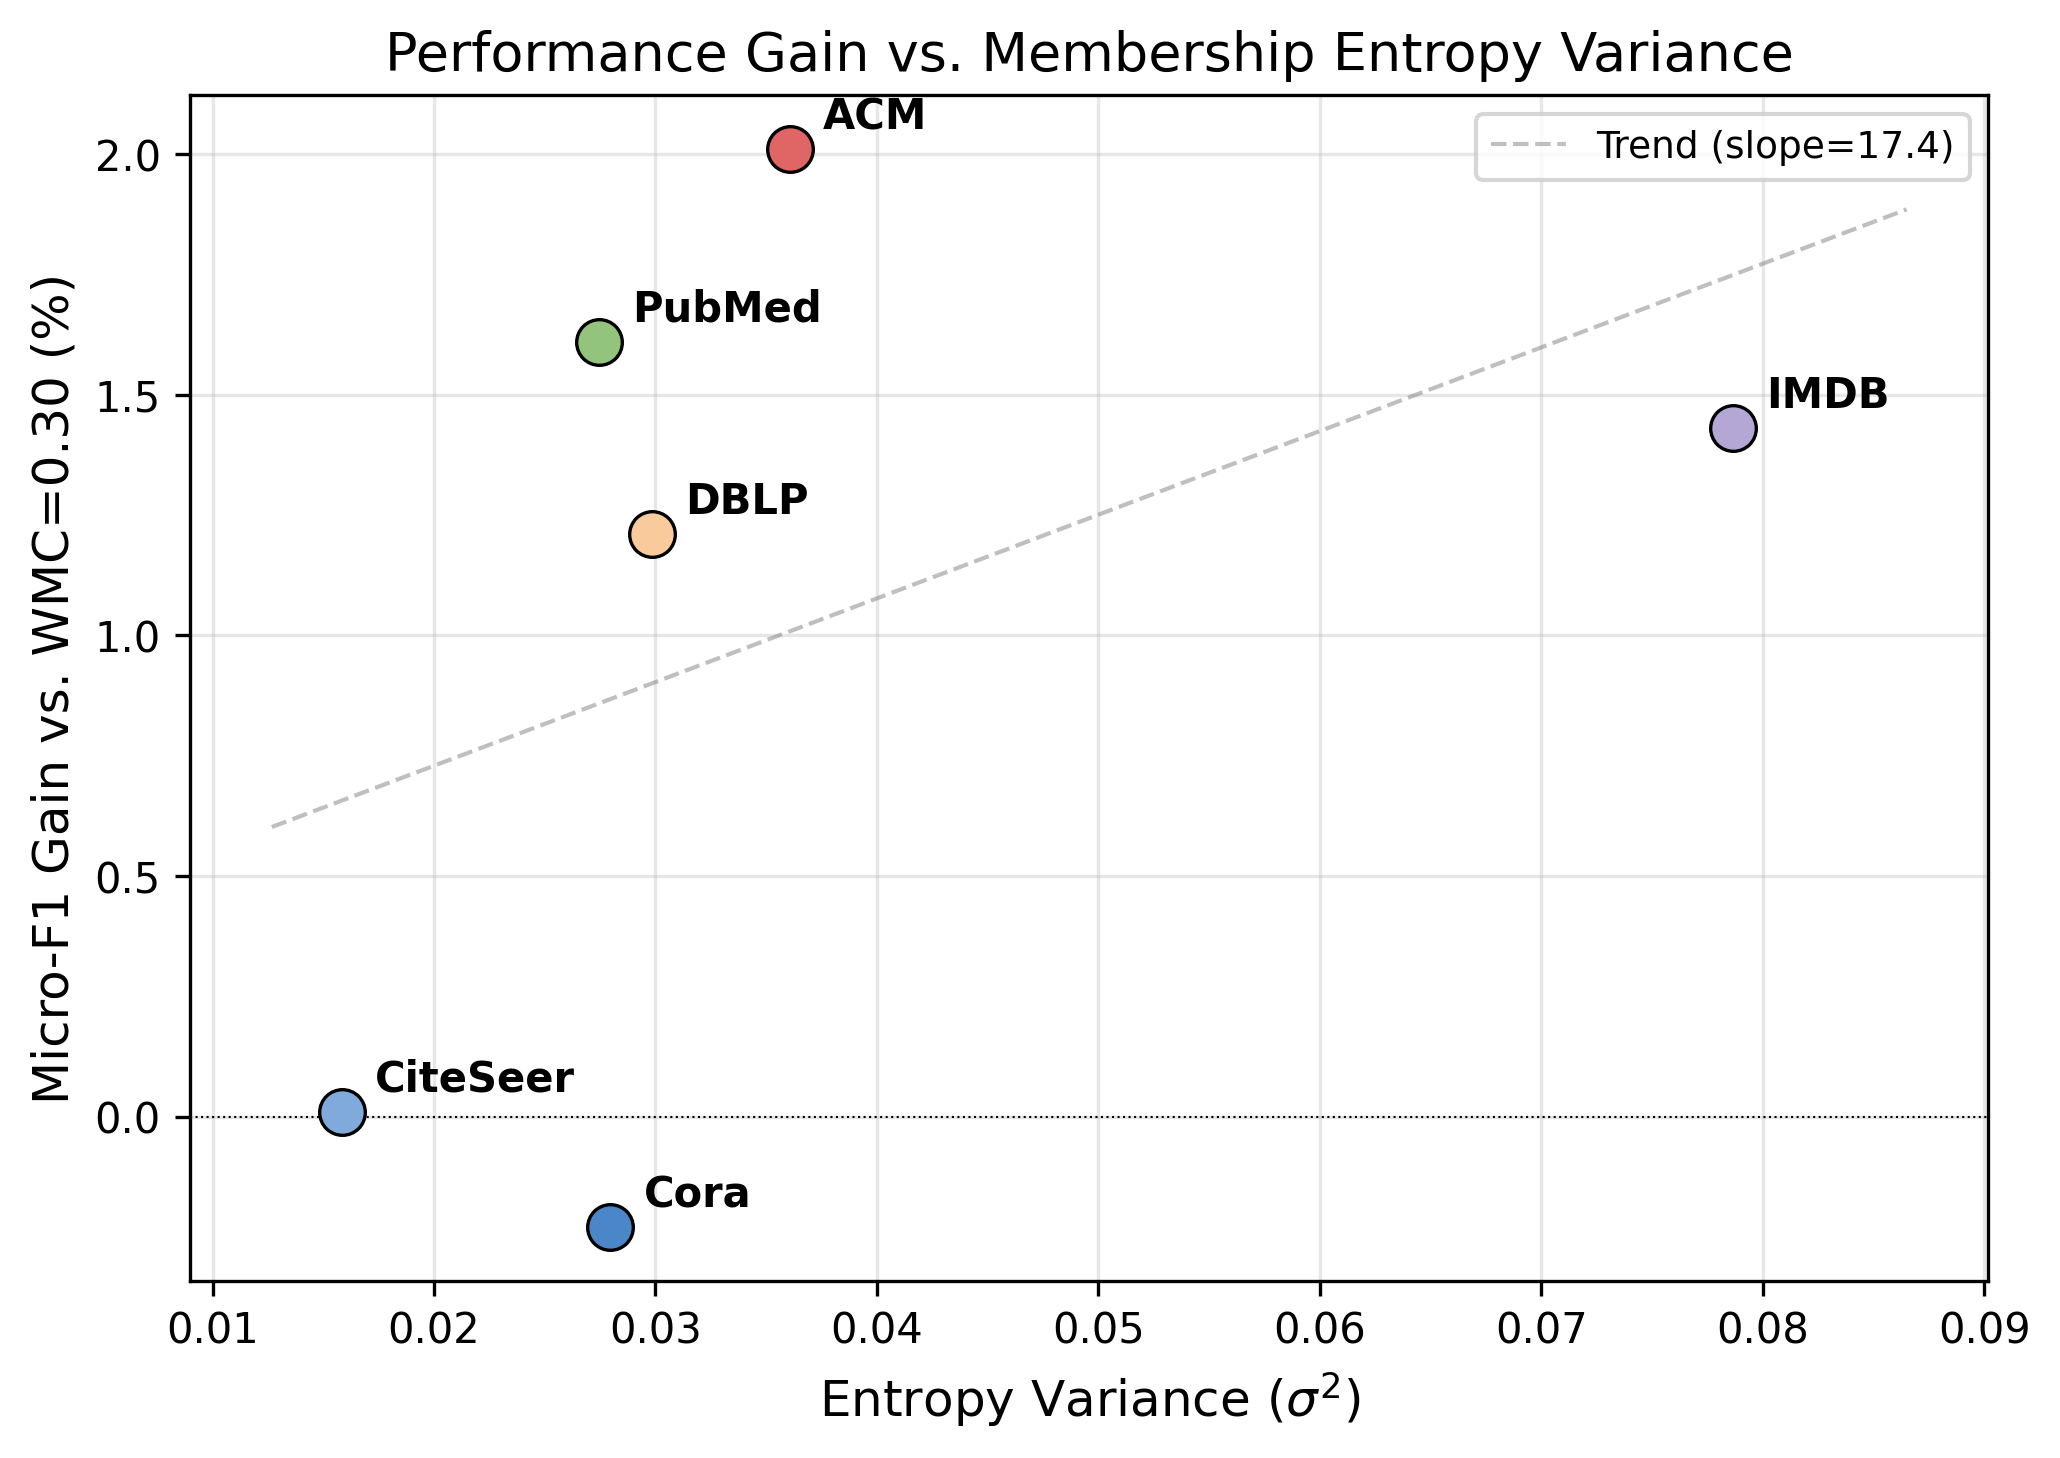
\includegraphics[width=0.75\textwidth]{figures/gain_vs_variance.png}
\caption{Performance gain (F1 improvement over WMC~=~0.30) vs.\ entropy variance ($\sigma^2$) for each dataset. PubMed and IMDB, with the highest entropy variance, show the largest gains. CiteSeer and ACM show negative or negligible gains.}
\label{fig:gain-variance}
\end{figure}

Ceiling effects (ACM) and very low ambiguity (CiteSeer) limit gains regardless of variance.


%%======================================================================
\section{Discussion}
\label{sec:discussion}
%%======================================================================

\subsection{The Ambiguity Hypothesis Is Validated}

The stratified analysis and correlation studies provide strong evidence that community-membership ambiguity identifies useful overlap nodes.
High-entropy nodes are 69--95\% overlap candidates, and they are assigned to 1.4--3.4 clusters on average.
The mechanism is intuitive: nodes with ambiguous memberships genuinely participate in multiple communities, and including them in multiple cluster subgraphs provides the GCN with richer training signals.
Low-entropy nodes, by contrast, are well-served by single-cluster training.

\subsection{Adaptive Thresholding Eliminates a Hyperparameter}

The primary practical contribution is the elimination of the WMC hyperparameter search.
Our fixed-WMC comparison (Table~\ref{tab:main-results}) shows that the optimal WMC varies across datasets: WMC~=~0.10 is best for CiteSeer, PubMed, and IMDB, while WMC~=~0.20--0.30 is best for Cora and DBLP.
Without adaptive methods, practitioners must search over WMC values---a costly process that requires retraining on each dataset.
Entropy-Adaptive with $\lambda = 0.50$ achieves competitive performance across all six datasets without per-dataset tuning.
Importantly, this is not a claim of universal superiority over well-tuned baselines, but rather a demonstration that a single universal configuration ($\mathrm{WMC}_{\mathrm{base}} = 0.3$, $\lambda = 0.5$) performs comparably to per-dataset tuned WMC, eliminating the need for grid search.
This is particularly valuable in scenarios where practitioners work with many graphs or where the optimal WMC is not known a priori.

\subsection{Performance Gains Are Modest but Real}

At matched overlap ratios, adaptive methods improve by +0.001 to +0.023 F1 over fixed baselines on four of six datasets.
The gains are real but modest, reflecting the fact that the original WMC already captures a substantial portion of the useful overlap signal.
Adaptive methods refine this signal by scaling the threshold based on node-level ambiguity, but the marginal improvement is bounded.
The contribution is not universal performance superiority over well-tuned baselines, but rather principled threshold selection that eliminates the tuning cost.

\subsection{Entropy vs.\ Margin: Complementary Signals}

Entropy-Adaptive and Margin-Adaptive perform similarly overall, but show different per-dataset preferences.
On datasets where ambiguity is primarily a top-two competition (DBLP, CiteSeer), Margin-Adaptive with low $\lambda$ performs best.
On datasets with richer multi-cluster ambiguity (PubMed, IMDB), Entropy-Adaptive or Margin-Adaptive with high $\lambda$ performs best.
The weak correlation between entropy and ambiguity on DBLP and CiteSeer ($r \approx -0.4$) confirms that these measures capture genuinely different aspects of the membership distribution.
A hybrid approach combining both signals could potentially improve robustness, though we leave this for future work.

\subsection{Practical Recommendations}

Based on our findings, we recommend:

\begin{enumerate}
  \item \textbf{Default configuration:} Entropy-Adaptive with $\mathrm{WMC}_{\mathrm{base}} = 0.3$ and $\lambda = 0.50$. This single configuration provides competitive performance across all tested datasets without per-dataset tuning.
  \item \textbf{When strong ambiguity is expected:} Increase $\lambda$ to 0.75 (as on IMDB).
  \item \textbf{When a tuned fixed WMC is available:} Adaptive methods are unlikely to significantly outperform it, but they provide a principled starting point that avoids the tuning cost.
\end{enumerate}


%%======================================================================
\section{Threats to Validity}
\label{sec:threats}
%%======================================================================

\paragraph{Dataset scope.}
We evaluate on six datasets, all of moderate size (2,363--19,717 nodes).
The largest graph, PubMed, has 19,717 nodes, which is small by modern standards.
Scaling to larger graphs (e.g., OGB benchmarks with millions of nodes) would strengthen the claims and test whether the ambiguity signal remains informative at scale.

\paragraph{Community detection method.}
All experiments use DANMF for membership estimation.
Different community detection methods may produce different membership distributions, potentially affecting the ambiguity signal.
The adaptive framework is method-agnostic in principle, but the specific entropy and margin values depend on the quality of the membership estimation.

\paragraph{Overlap ratio range.}
Our experiments fix $\mathrm{WMC}_{\mathrm{base}} = 0.3$ and vary only $\lambda$.
Different base WMC values could shift the overlap ratio range and affect the relative advantage of adaptive methods.
We chose $\mathrm{WMC}_{\mathrm{base}} = 0.3$ because it is the default in the original OCGCN.

\paragraph{Statistical power.}
With 10 seeds per configuration, we have limited power to detect small effect sizes.
The marginal significance on DBLP ($p = 0.052$) and non-significance on Cora, PubMed, and ACM could reflect insufficient power rather than true null effects.
Larger-scale experiments with more seeds would clarify this.

\paragraph{Single GCN architecture.}
We use a fixed 3-layer GCN with 64 hidden units.
Different architectures (deeper/wider GCNs, attention-based models) might interact differently with overlap assignment.
The adaptive thresholding is architecture-agnostic, but the magnitude of its benefit may vary.


%%======================================================================
\section{Conclusion}
\label{sec:conclusion}
%%======================================================================

This paper introduces adaptive overlap thresholding for Overlapping Cluster-GCN, replacing the global WMC threshold with node-specific thresholds derived from community-membership ambiguity.
Two variants are proposed: Entropy-Adaptive WMC, which scales the threshold by normalized membership entropy, and Margin-Adaptive WMC, which scales by the ambiguity of the top-two membership gap.
Both methods replace per-dataset WMC grid search with a single universal configuration ($\mathrm{WMC}_{\mathrm{base}} = 0.3$, $\lambda = 0.5$) that achieves competitive performance across six benchmark graphs.

The core hypothesis---that membership ambiguity identifies useful overlap nodes---is validated through stratified analysis showing that high-entropy nodes are 69--95\% overlap candidates, with strong correlations between entropy and cluster count on all datasets.
Performance gains from adaptive thresholding are modest but real: at matched overlap ratios, adaptive methods improve by +0.001 to +0.023 F1 over fixed baselines on four of six datasets, with Entropy-Adaptive achieving the highest overlap efficiency on Cora and PubMed.

The practical value of adaptive thresholding is the removal of the WMC hyperparameter search, a process that varies across datasets and requires costly retraining.
Entropy-Adaptive with $\lambda = 0.50$ provides a reasonable default that works well across diverse graph types.
Future work should explore hybrid entropy-margin methods, scaling to larger graphs, and theoretical analysis of the overlap quality bound.


%%======================================================================
%% References
%%======================================================================
\begin{thebibliography}{99}

\bibitem{kipf2017semi}
T.~N. Kipf and M.~Welling,
``Semi-supervised classification with graph convolutional networks,''
in \emph{Proc. Int. Conf. on Learning Representations (ICLR)}, 2017.

\bibitem{Cluster-GCN}
W.-L. Chiang, X.~Liu, S.~Si, Y.~Li, S.~Bengio, and C.-J. Hsieh,
``Cluster-GCN: An efficient algorithm for training deep and large graph convolutional networks,''
in \emph{Proc. ACM SIGKDD Int. Conf. on Knowledge Discovery and Data Mining}, 2019, pp.~257--266.

\bibitem{GraphSAGE}
W.~L. Hamilton, Z.~Ying, and J.~Leskovec,
``Inductive representation learning on large graphs,''
in \emph{Advances in Neural Information Processing Systems (NeurIPS)}, 2017, pp.~1024--1034.

\bibitem{chen2018fastgcn}
J.~Chen, T.~Ma, and C.~Xiao,
``FastGCN: Fast learning with graph convolutional networks via importance sampling,''
in \emph{Proc. Int. Conf. on Learning Representations (ICLR)}, 2018.

\bibitem{dai2018learning}
H.~Dai, Z.~Li, T.~Tian, X.~Zhu, and L.~Song,
``Stochastic training of graph convolutional networks with variance reduction,''
in \emph{Proc. Int. Conf. on Machine Learning (ICML)}, 2018, pp.~942--950.

\bibitem{vel2018graph}
P.~Veli\v{c}kovi\'{c}, G.~Cucurull, A.~Casanova, A.~Romero, P.~Li\`{o}, and Y.~Bengio,
``Graph attention networks,''
in \emph{Proc. Int. Conf. on Learning Representations (ICLR)}, 2018.

\bibitem{Amintoosi2022}
M.~Amintoosi,
``Overlapping clusters in cluster convolutional networks,''
\emph{Journal of Applied Analysis and Computation}, vol.~12, no.~3, pp.~1173--1189, 2022.

\bibitem{DANMF}
Q.~M.~A. {Tran}, H.~Duong, and D.~Phung,
``DANMF: Deep adversarial non-negative matrix factorization for community detection,''
\emph{arXiv preprint arXiv:1810.11496}, 2018.

\bibitem{Shang2014}
Y.~Shang, L.~Zhao, J.~Xu, and L.~Gao,
``Overlapping community detection based on modularity and labeled propagation,''
\emph{Physics Procedia}, vol.~57, pp.~75--83, 2014.

\end{thebibliography}

\end{document}
